% Supplementary Materials — standalone file
% Companion to main.tex (When Does Temperature Scaling Pay Off in Cross-Corpus ECG Transfer?)
\documentclass[12pt]{article}
\usepackage[a4paper,margin=2.5cm]{geometry}
\usepackage{graphicx,booktabs,amsmath,amssymb}
\usepackage[utf8]{inputenc}
\usepackage{caption}
\usepackage{hyperref}
\captionsetup{font=small}
\begin{document}
\title{Supplementary Materials:\\ Per-seed reliability diagrams for the 60-experiment transfer grid}
\author{}
\date{}
\maketitle
\section*{Supplementary Materials: S1.\ Per-seed reliability diagrams}
\label{sec:supplementary}
% ============================================================================
This section catalogs the 60 per-seed reliability diagrams referenced
in the main text. Each figure shows the calibration curve, reliability
diagram, and $\Delta$ECE bar plot for one of the 60 seed experiments
(6 transfer pairs $\times$ 2 architectures $\times$ 5 seeds). Figures
are named \texttt{fig\_reliability\_supp\_\{pair\}\_\{arch\}\_seed\{s\}.pdf}
and are included as external files with the submission.

\subsection*{S1.\ Per-seed reliability diagrams}
\label{sec:supp-reliability}

The 60 figures are organized by transfer pair and architecture. Each
figure corresponds to one row in the master results table and provides
the visual calibration evidence underlying the $\Delta$ECE values
reported in the main text. For each direction, ResNet1D and
InceptionTime reliability diagrams are shown across seeds 42--46.

\subsubsection*{S1.1.\ Chapman$\rightarrow$CPSC}

\begin{figure}[h]
\centering
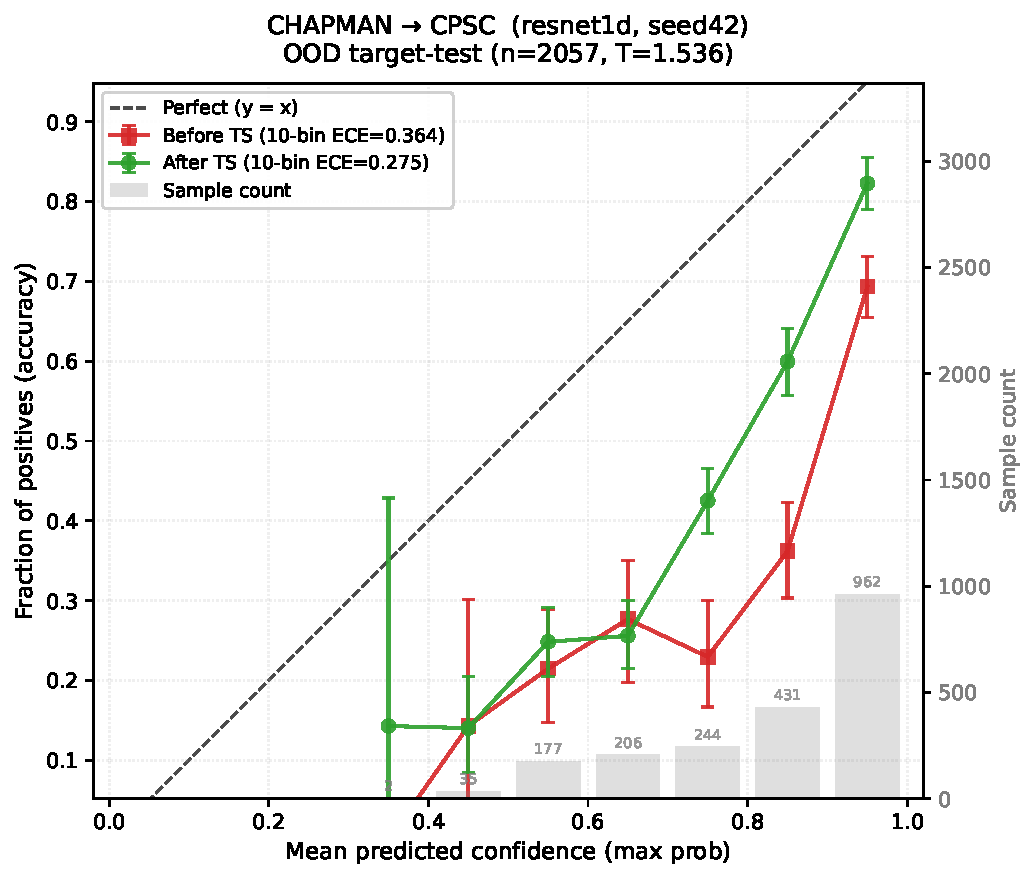
\includegraphics[width=0.32\textwidth]{figures/fig_reliability_supp_chapman_cpsc_resnet1d_seed42.pdf}
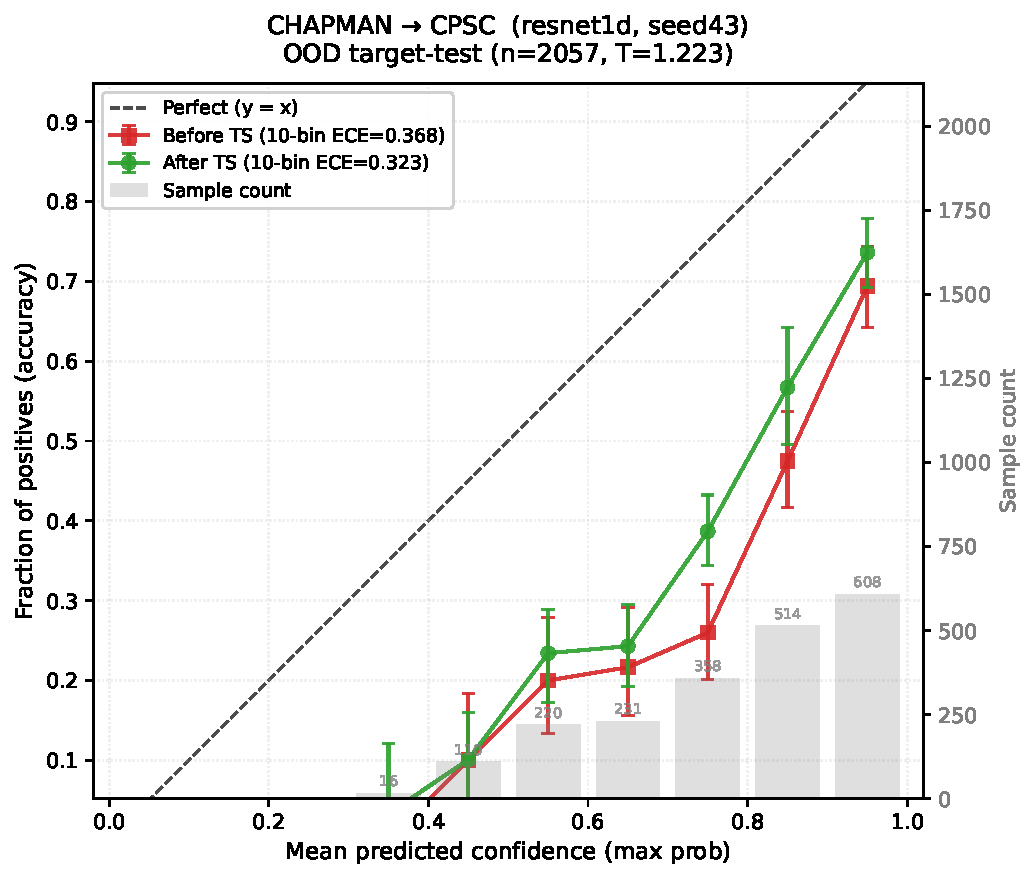
\includegraphics[width=0.32\textwidth]{figures/fig_reliability_supp_chapman_cpsc_resnet1d_seed43.pdf}
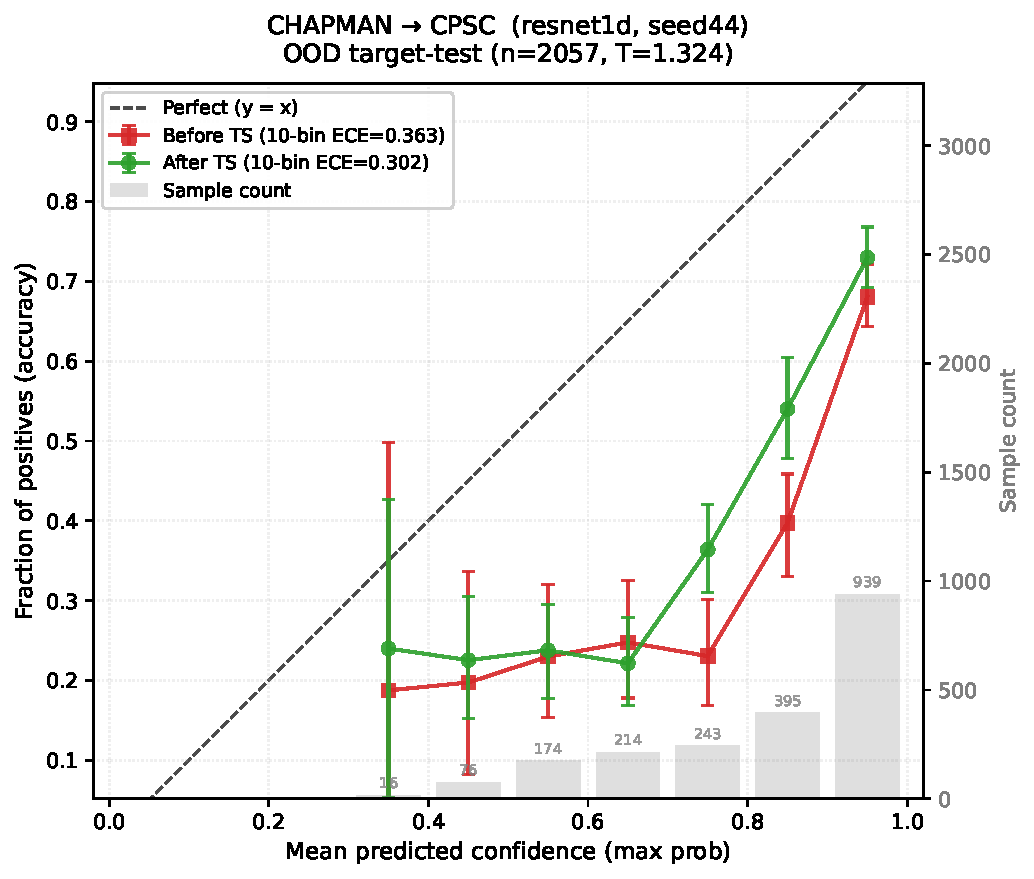
\includegraphics[width=0.32\textwidth]{figures/fig_reliability_supp_chapman_cpsc_resnet1d_seed44.pdf}
\caption{Chapman$\to$CPSC reliability diagrams: ResNet1D seeds 42--44.}
\end{figure}

\begin{figure}[h]
\centering
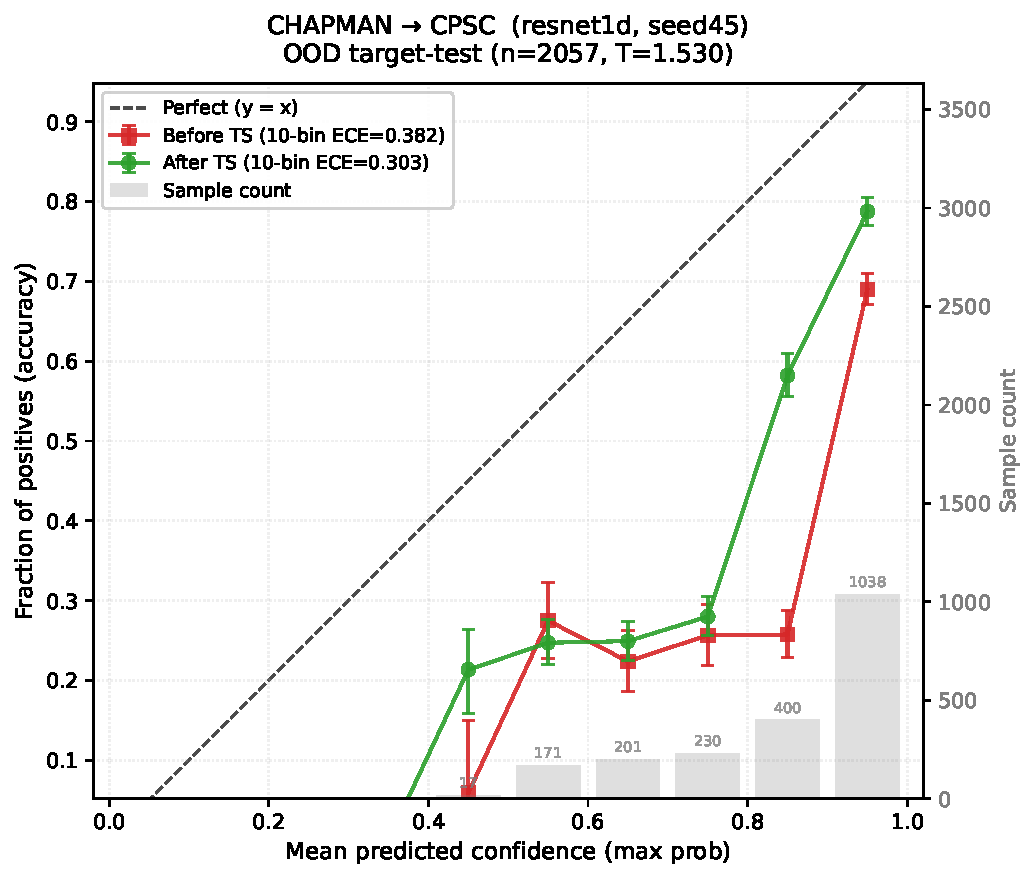
\includegraphics[width=0.45\textwidth]{figures/fig_reliability_supp_chapman_cpsc_resnet1d_seed45.pdf}
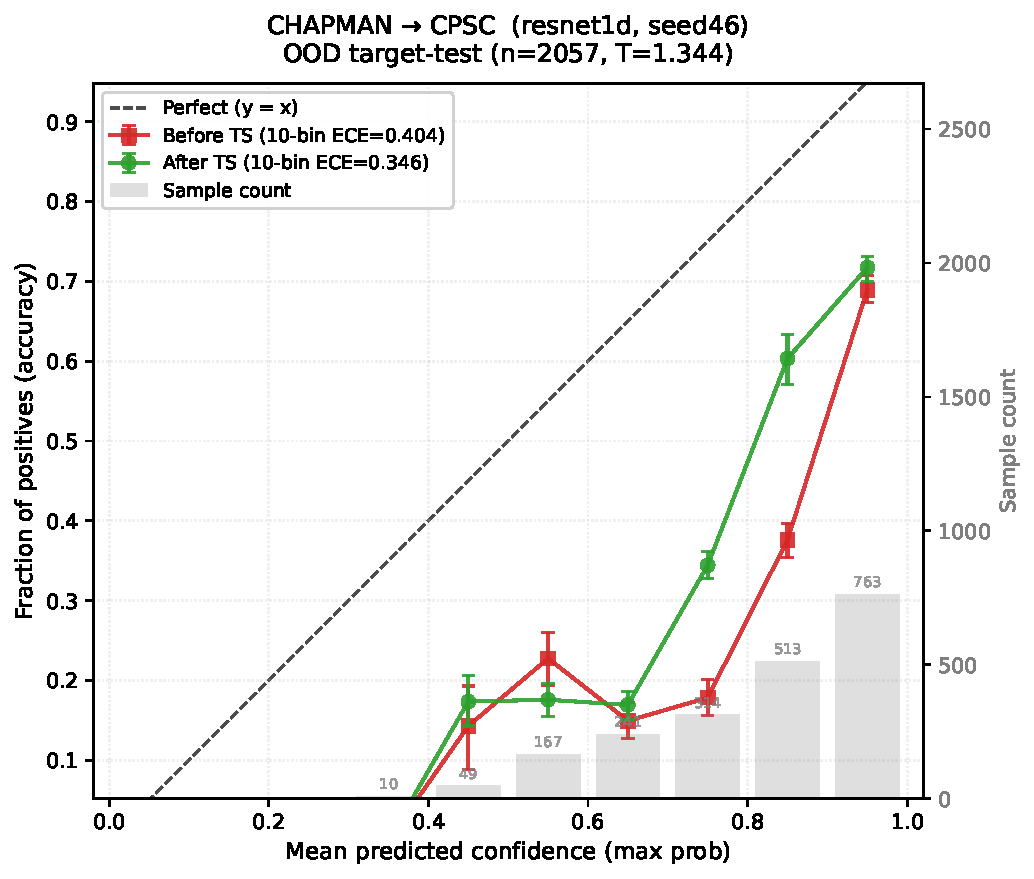
\includegraphics[width=0.45\textwidth]{figures/fig_reliability_supp_chapman_cpsc_resnet1d_seed46.pdf}
\caption{Chapman$\to$CPSC reliability diagrams: ResNet1D seeds 45--46.}
\end{figure}

\begin{figure}[h]
\centering
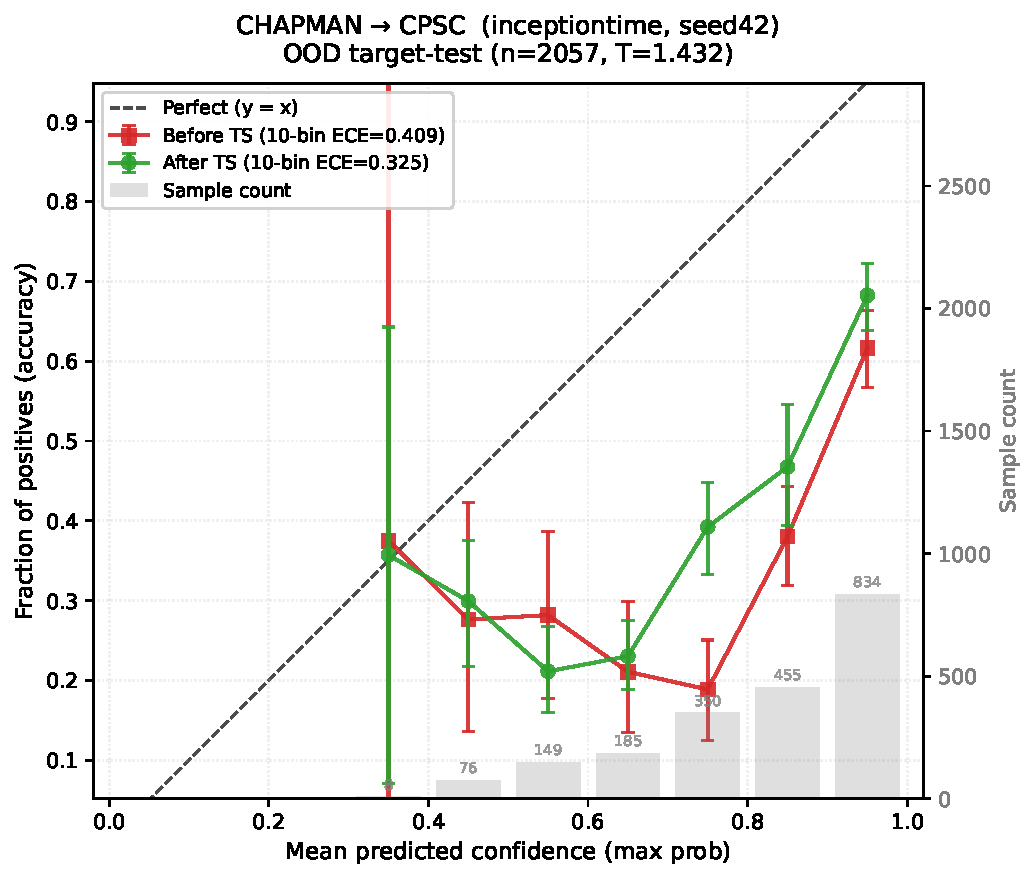
\includegraphics[width=0.32\textwidth]{figures/fig_reliability_supp_chapman_cpsc_inceptiontime_seed42.pdf}
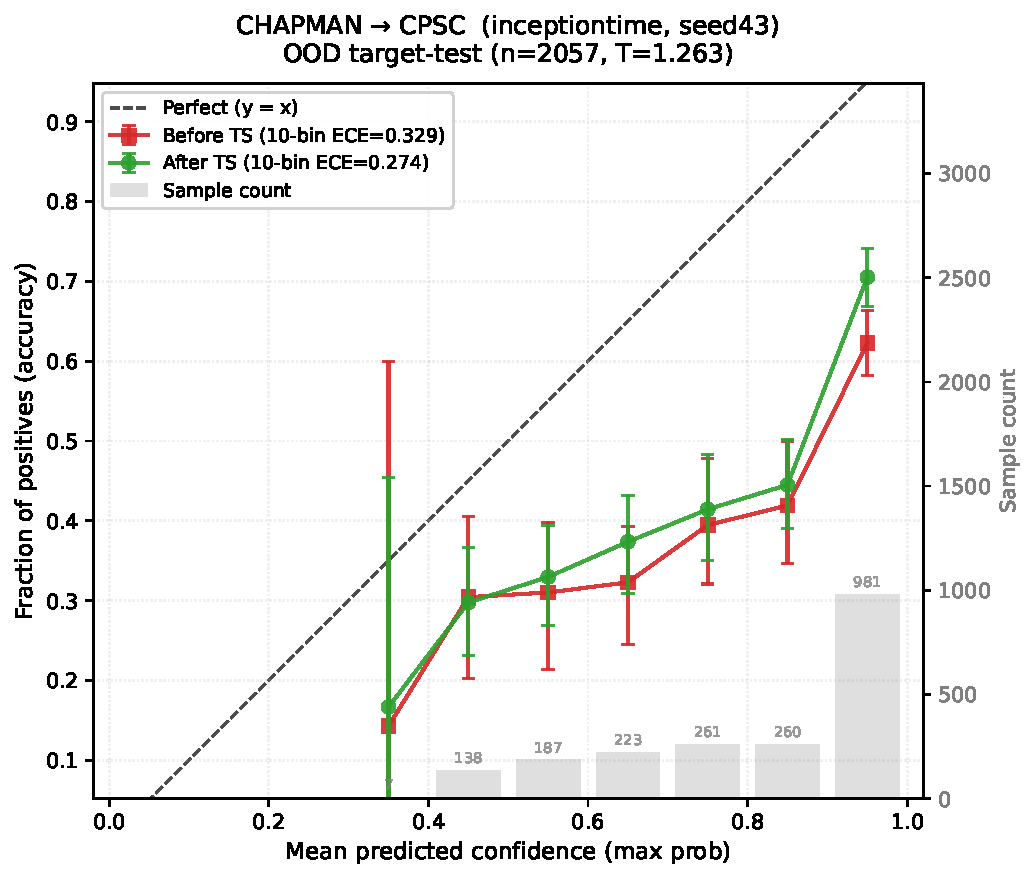
\includegraphics[width=0.32\textwidth]{figures/fig_reliability_supp_chapman_cpsc_inceptiontime_seed43.pdf}
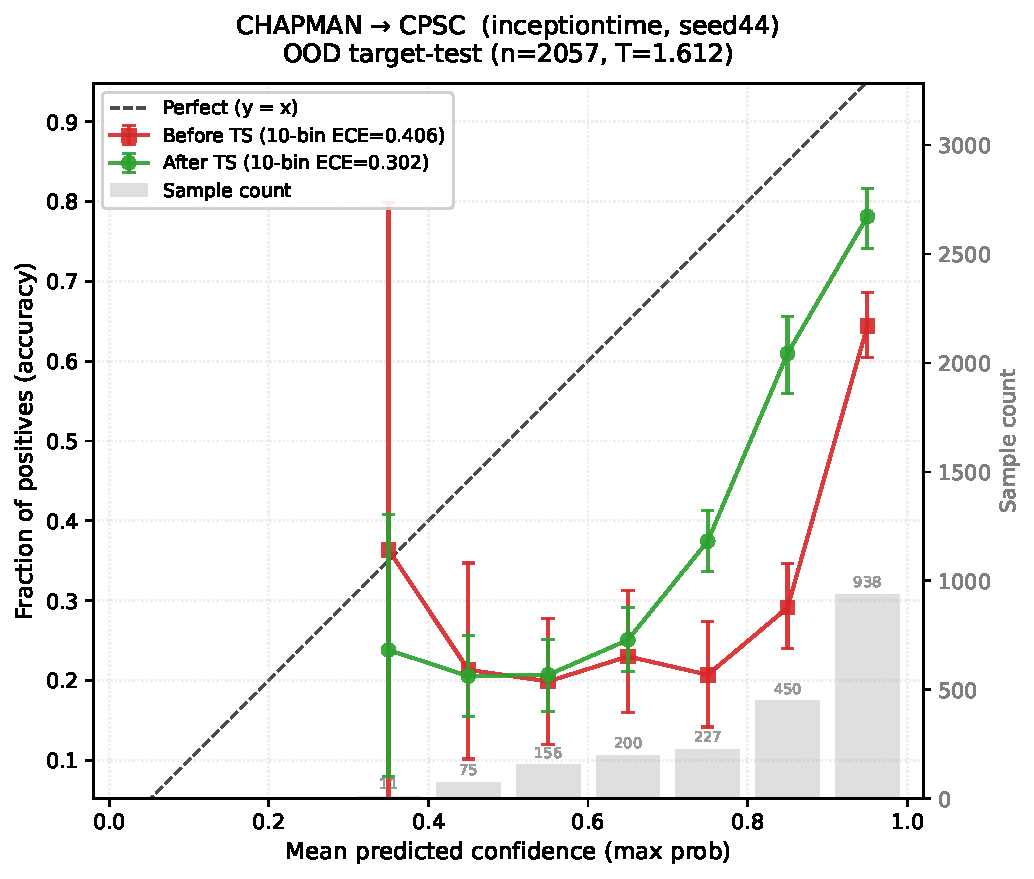
\includegraphics[width=0.32\textwidth]{figures/fig_reliability_supp_chapman_cpsc_inceptiontime_seed44.pdf}
\caption{Chapman$\to$CPSC reliability diagrams: InceptionTime seeds 42--44.}
\end{figure}

\begin{figure}[h]
\centering
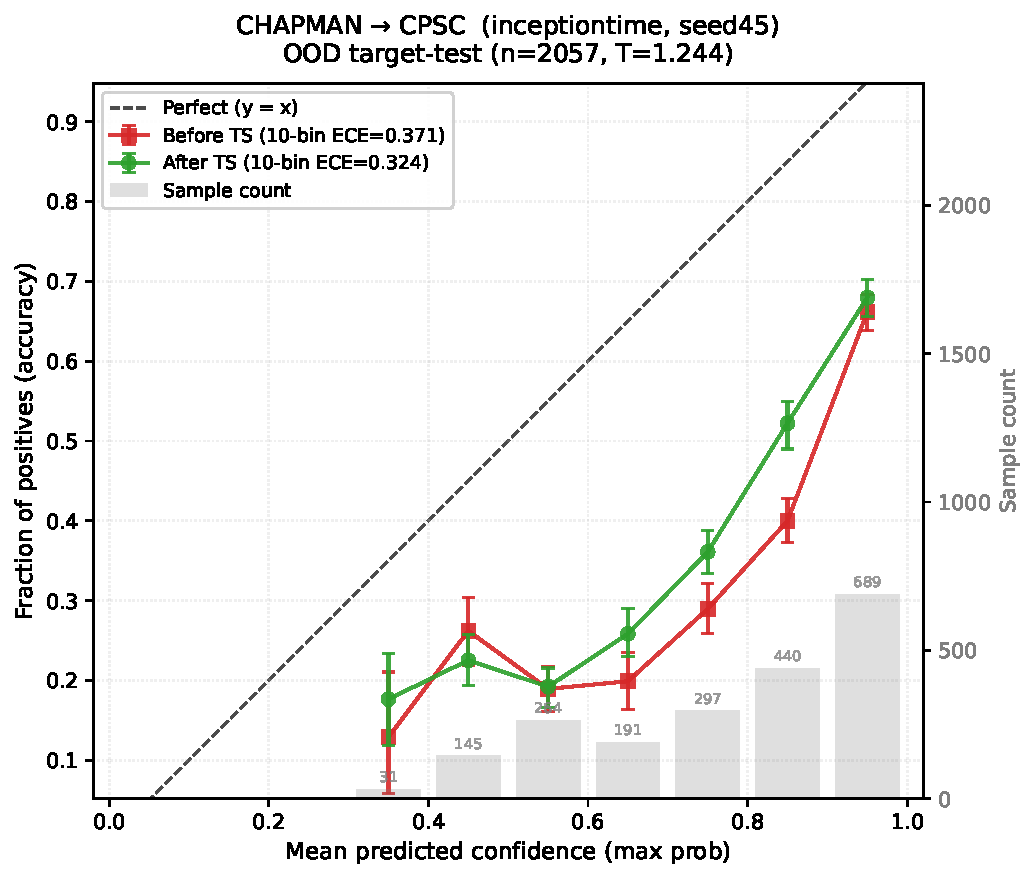
\includegraphics[width=0.45\textwidth]{figures/fig_reliability_supp_chapman_cpsc_inceptiontime_seed45.pdf}
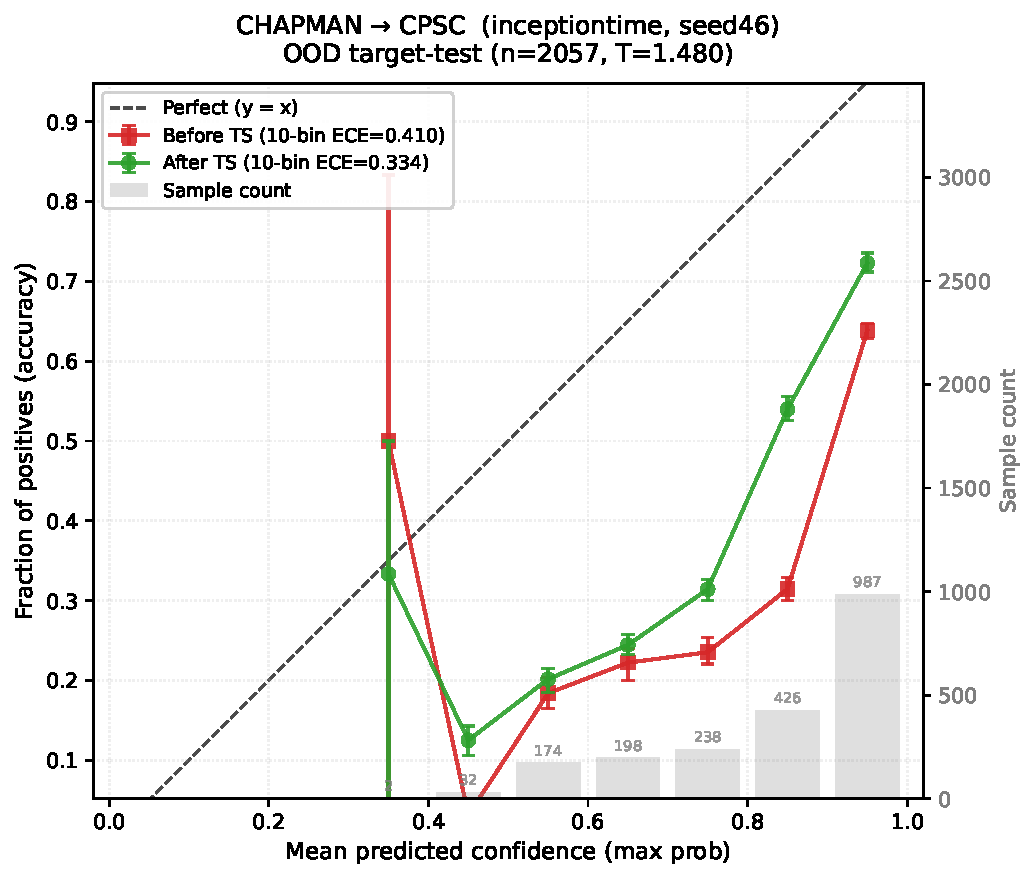
\includegraphics[width=0.45\textwidth]{figures/fig_reliability_supp_chapman_cpsc_inceptiontime_seed46.pdf}
\caption{Chapman$\to$CPSC reliability diagrams: InceptionTime seeds 45--46.}
\end{figure}

\subsubsection*{S1.2.\ Chapman$\rightarrow$PTB-XL}

\begin{figure}[h]
\centering
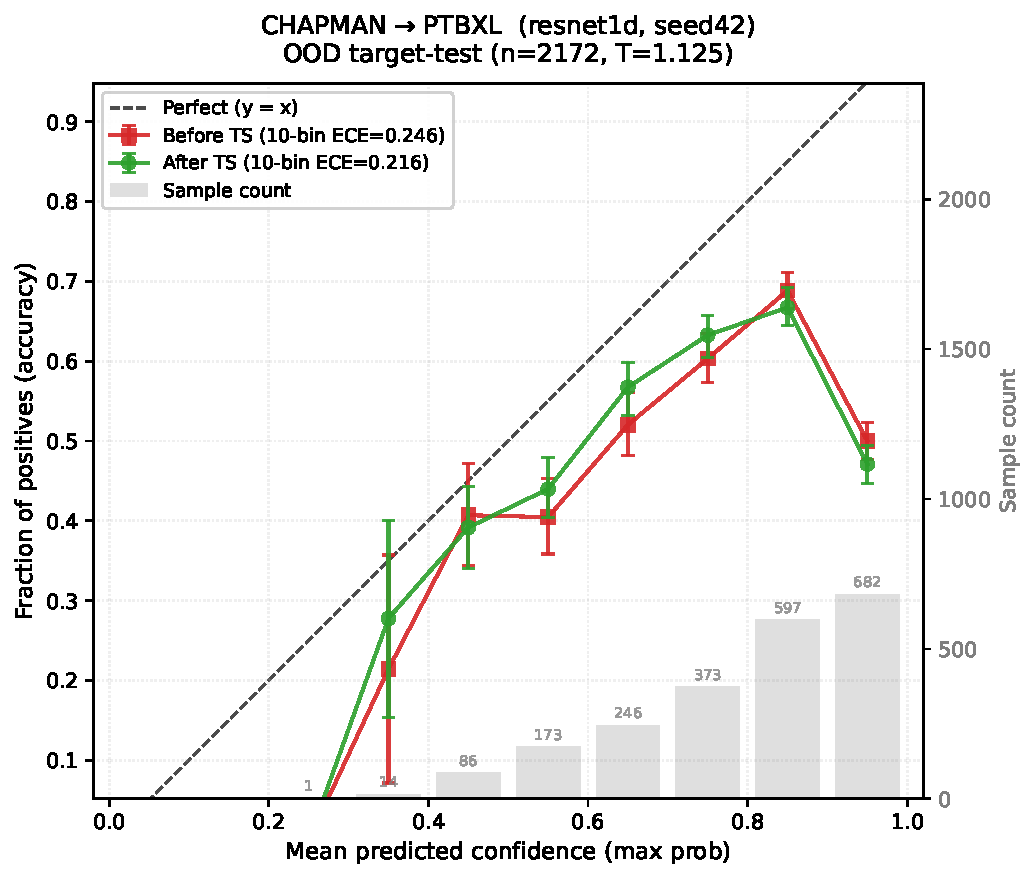
\includegraphics[width=0.32\textwidth]{figures/fig_reliability_supp_chapman_ptbxl_resnet1d_seed42.pdf}
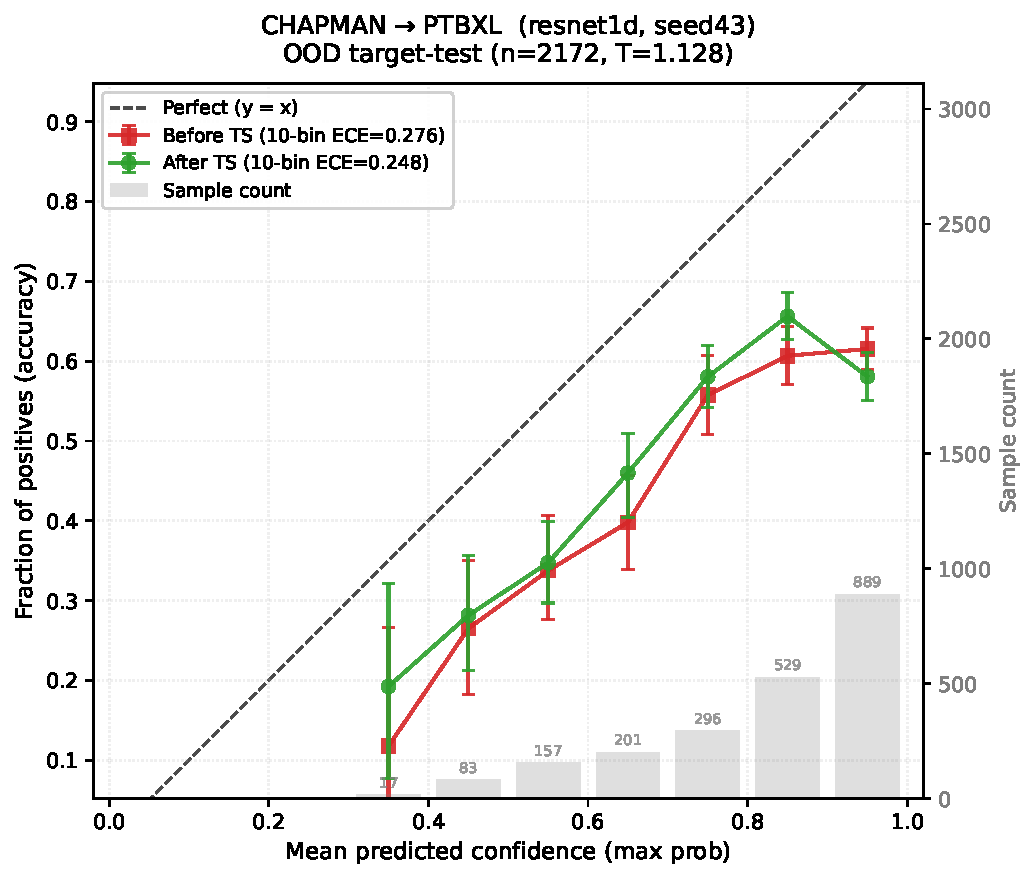
\includegraphics[width=0.32\textwidth]{figures/fig_reliability_supp_chapman_ptbxl_resnet1d_seed43.pdf}
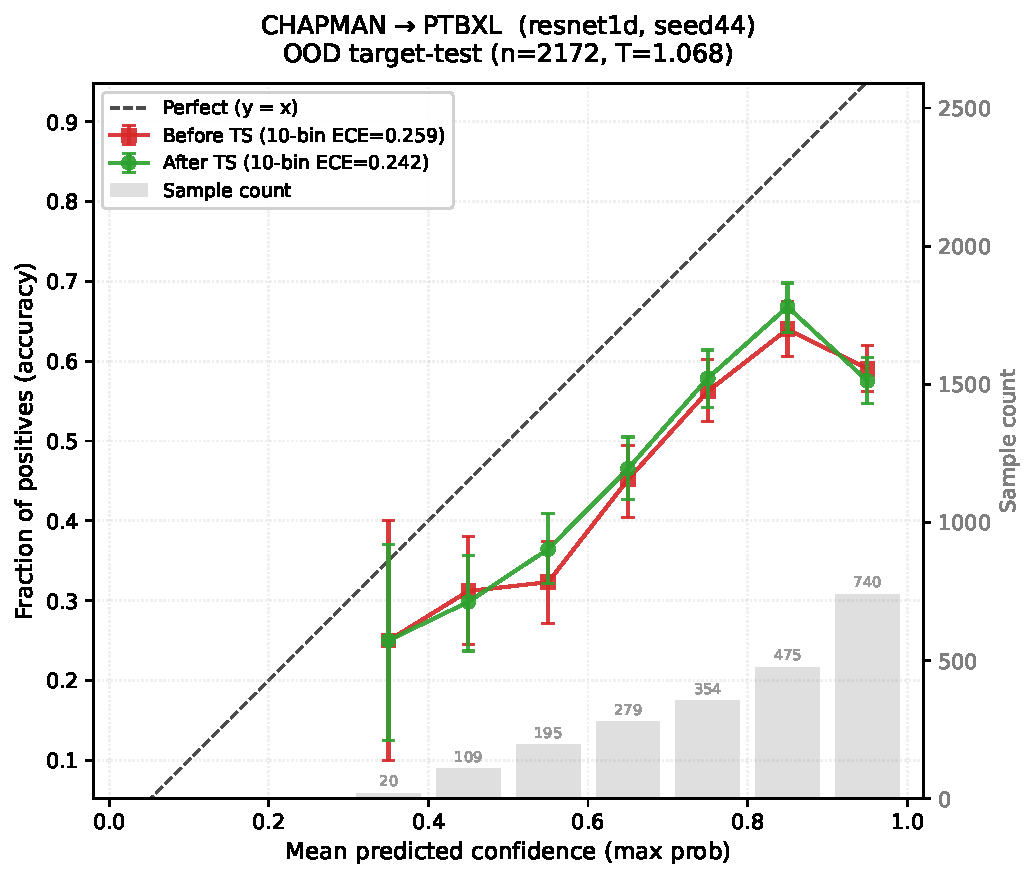
\includegraphics[width=0.32\textwidth]{figures/fig_reliability_supp_chapman_ptbxl_resnet1d_seed44.pdf}
\caption{Chapman$\to$PTB-XL reliability diagrams: ResNet1D seeds 42--44.}
\end{figure}

\begin{figure}[h]
\centering
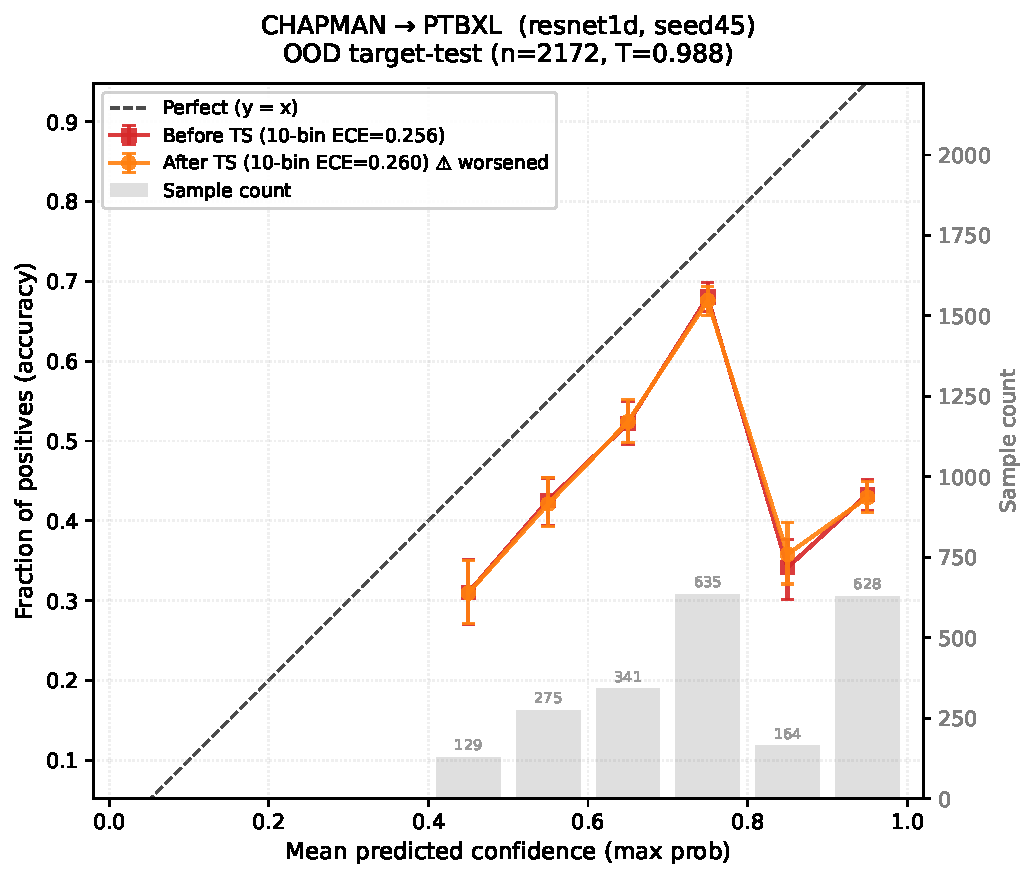
\includegraphics[width=0.45\textwidth]{figures/fig_reliability_supp_chapman_ptbxl_resnet1d_seed45.pdf}
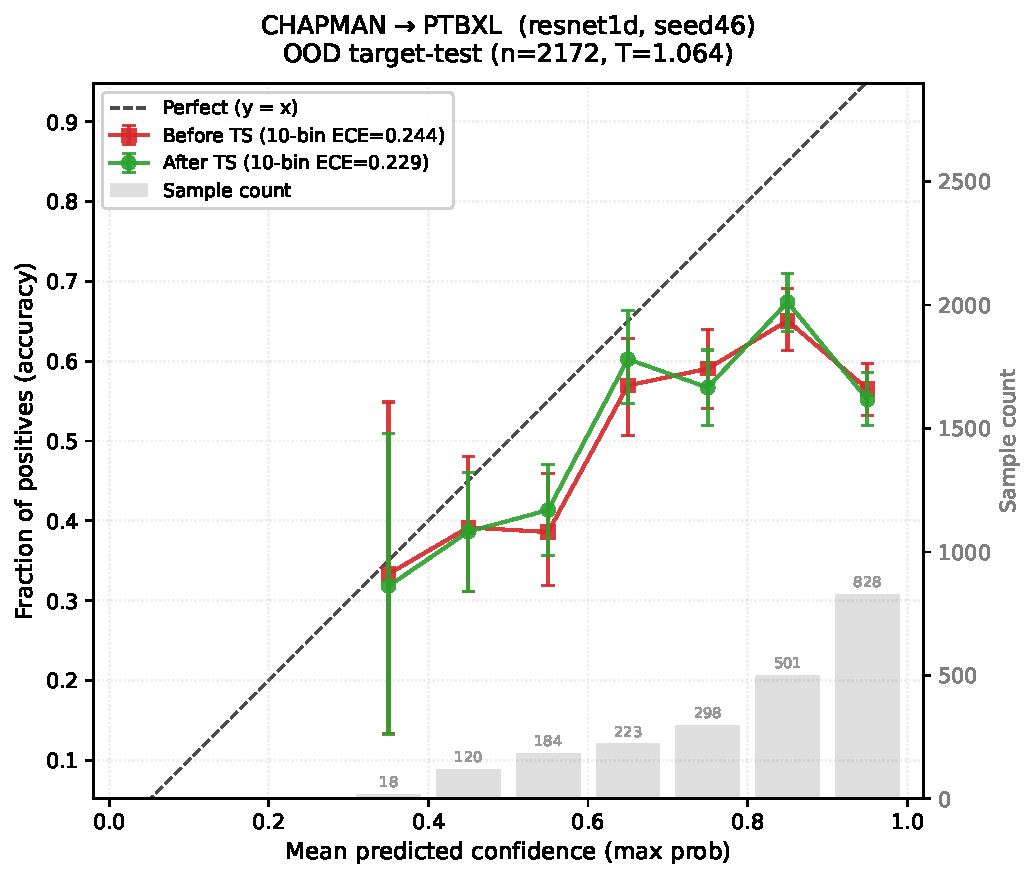
\includegraphics[width=0.45\textwidth]{figures/fig_reliability_supp_chapman_ptbxl_resnet1d_seed46.pdf}
\caption{Chapman$\to$PTB-XL reliability diagrams: ResNet1D seeds 45--46.}
\end{figure}

\begin{figure}[h]
\centering
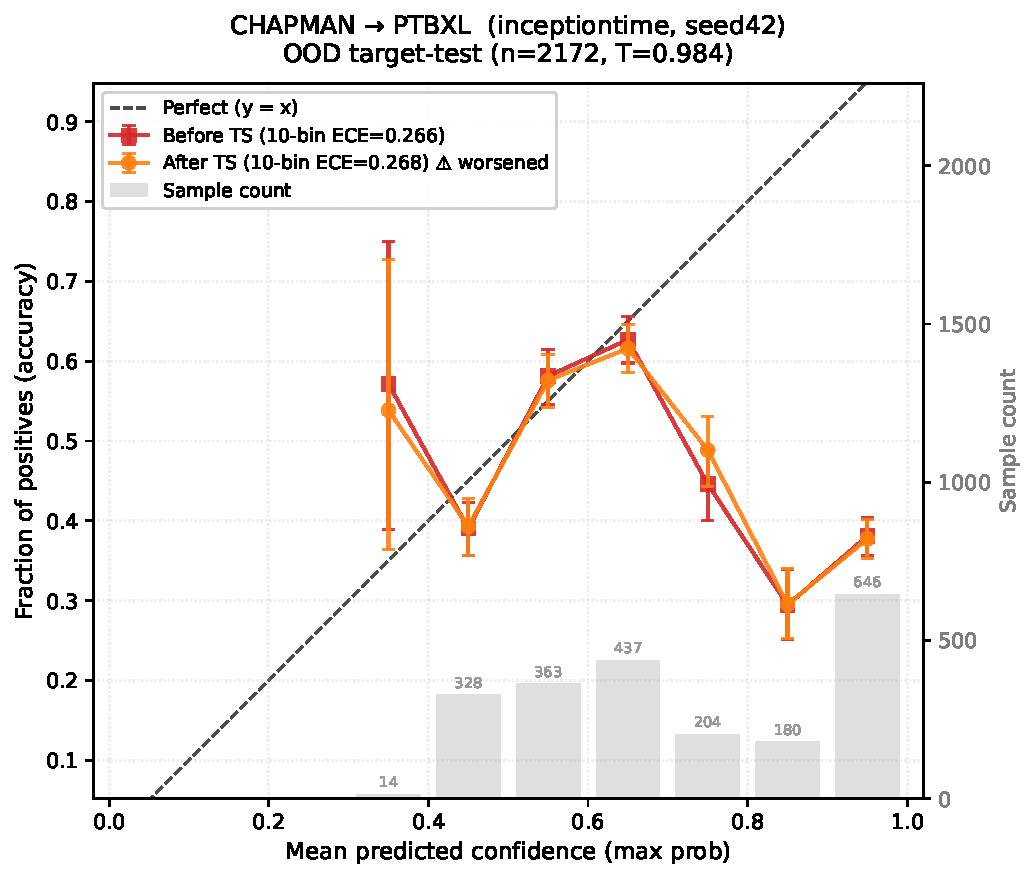
\includegraphics[width=0.32\textwidth]{figures/fig_reliability_supp_chapman_ptbxl_inceptiontime_seed42.pdf}
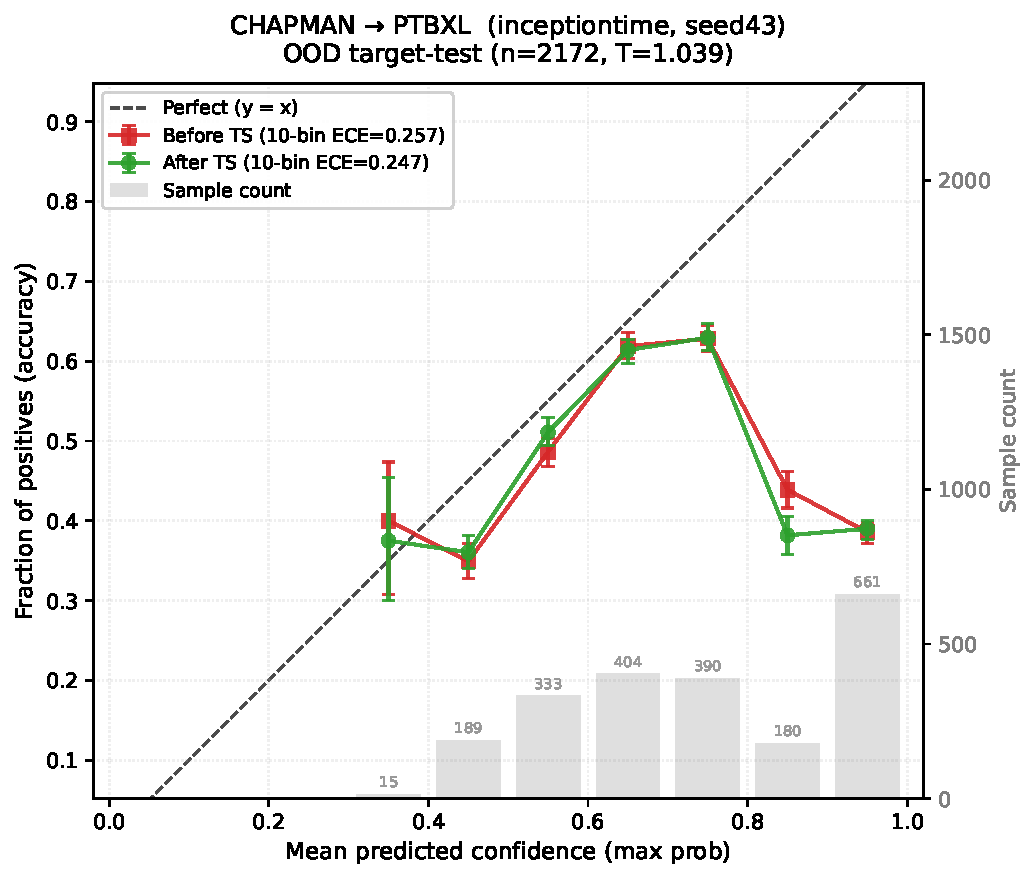
\includegraphics[width=0.32\textwidth]{figures/fig_reliability_supp_chapman_ptbxl_inceptiontime_seed43.pdf}
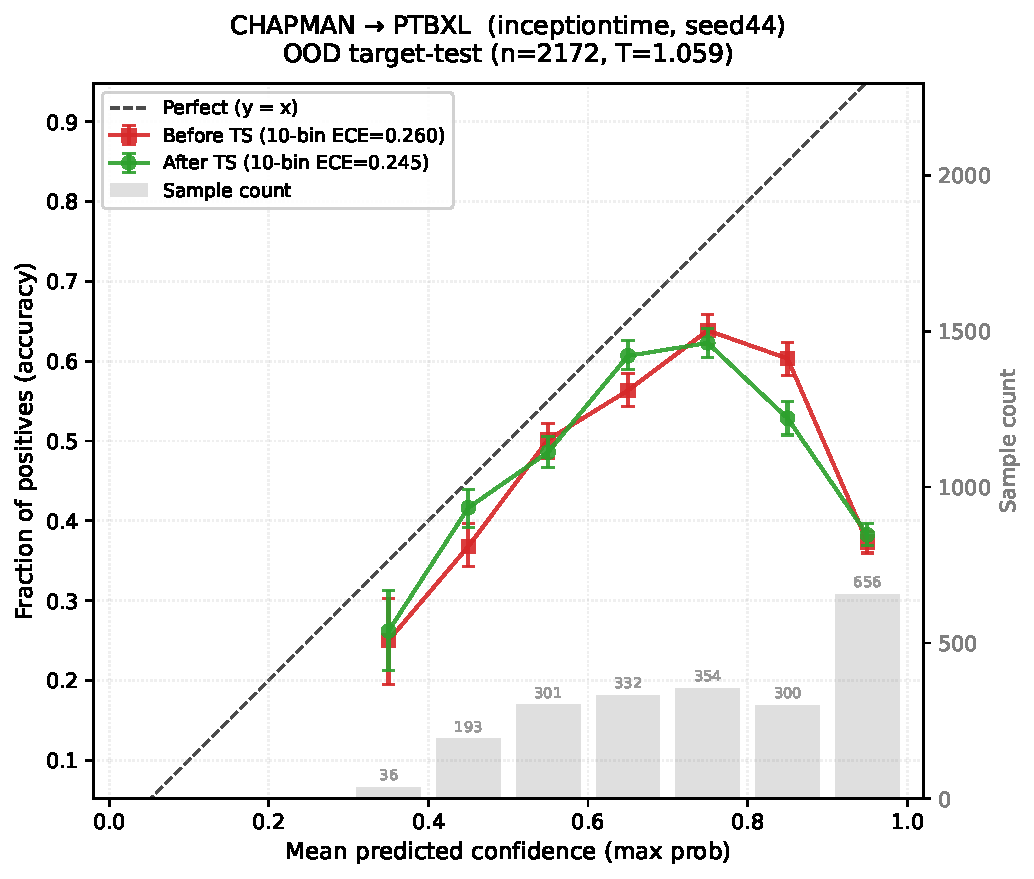
\includegraphics[width=0.32\textwidth]{figures/fig_reliability_supp_chapman_ptbxl_inceptiontime_seed44.pdf}
\caption{Chapman$\to$PTB-XL reliability diagrams: InceptionTime seeds 42--44.}
\end{figure}

\begin{figure}[h]
\centering
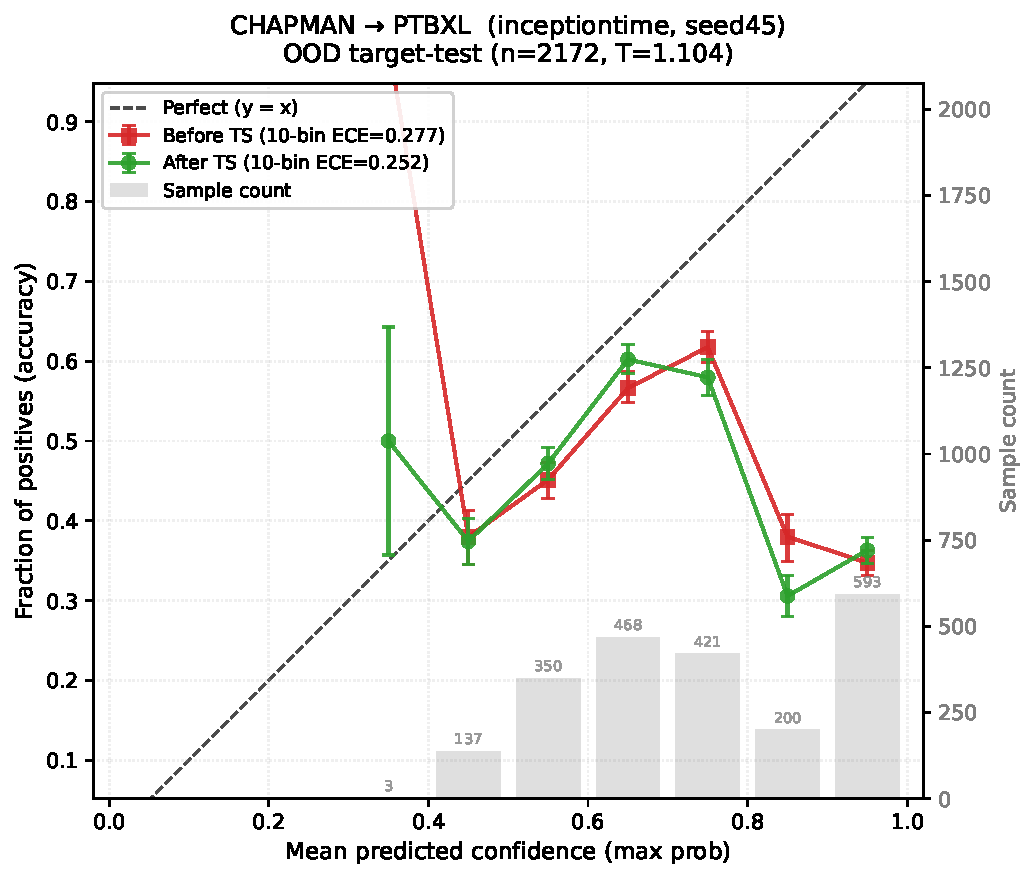
\includegraphics[width=0.45\textwidth]{figures/fig_reliability_supp_chapman_ptbxl_inceptiontime_seed45.pdf}
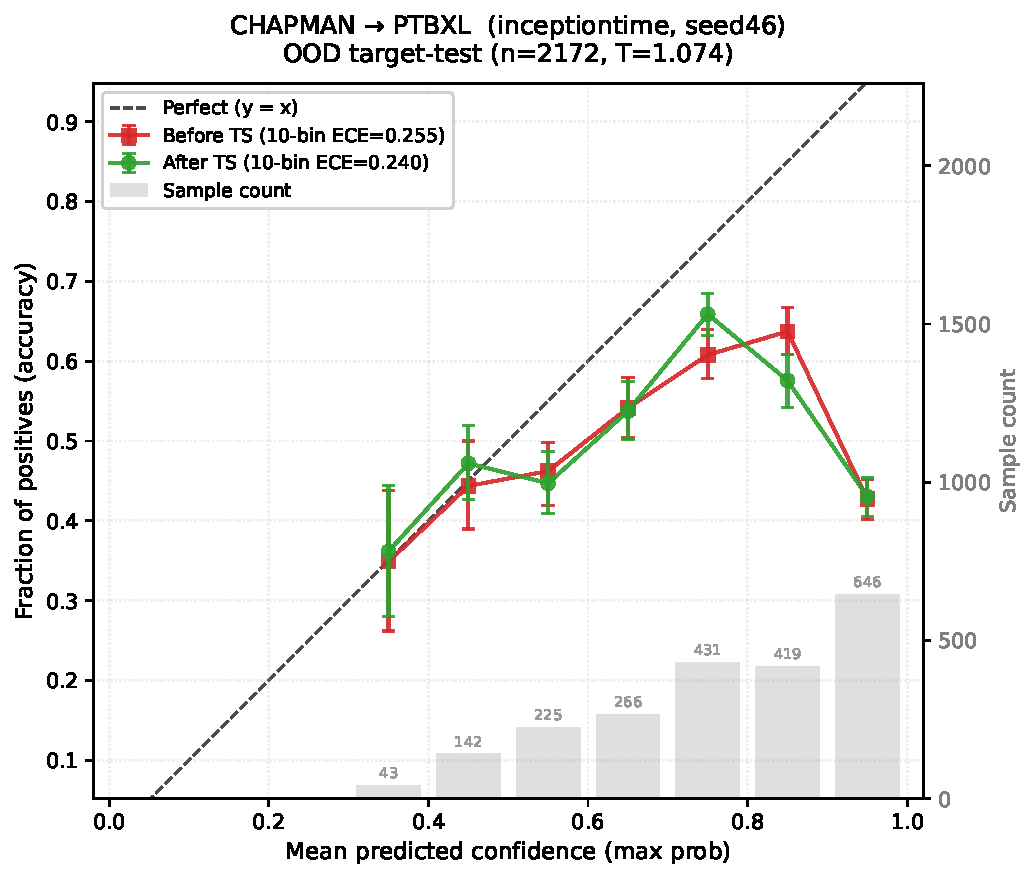
\includegraphics[width=0.45\textwidth]{figures/fig_reliability_supp_chapman_ptbxl_inceptiontime_seed46.pdf}
\caption{Chapman$\to$PTB-XL reliability diagrams: InceptionTime seeds 45--46.}
\end{figure}

\subsubsection*{S1.3.\ CPSC$\rightarrow$Chapman}

\begin{figure}[h]
\centering
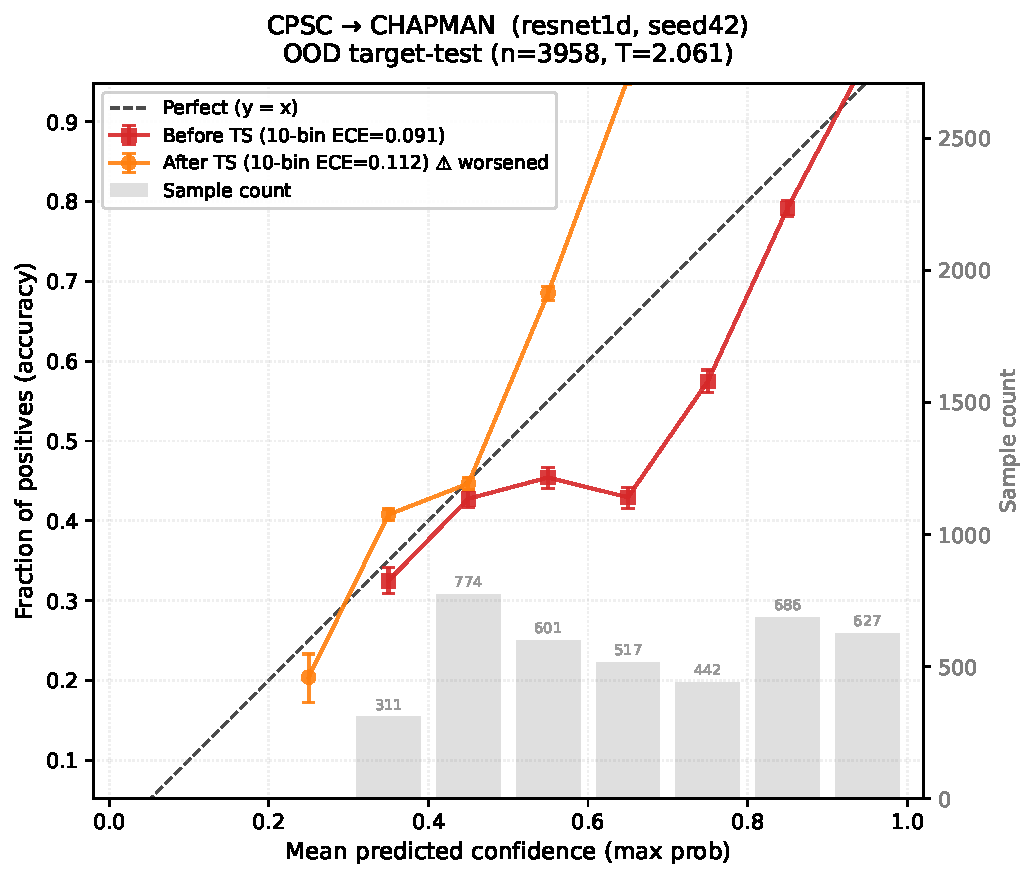
\includegraphics[width=0.32\textwidth]{figures/fig_reliability_supp_cpsc_chapman_resnet1d_seed42.pdf}
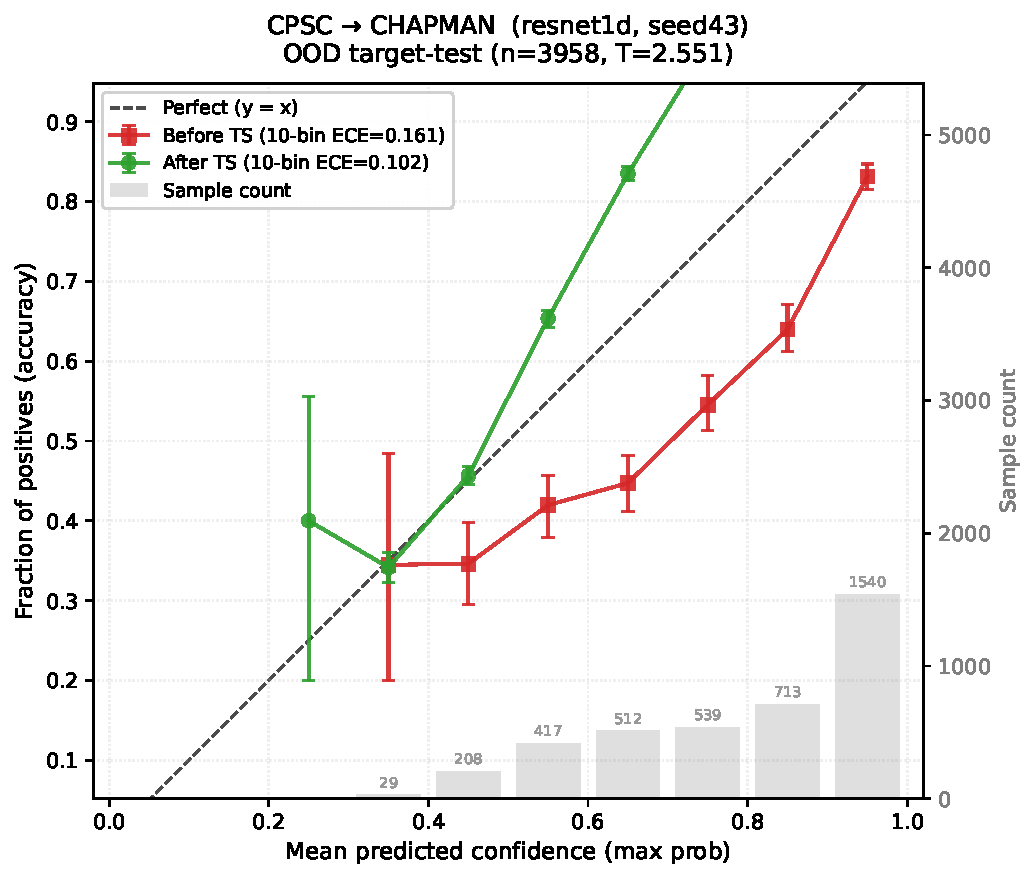
\includegraphics[width=0.32\textwidth]{figures/fig_reliability_supp_cpsc_chapman_resnet1d_seed43.pdf}
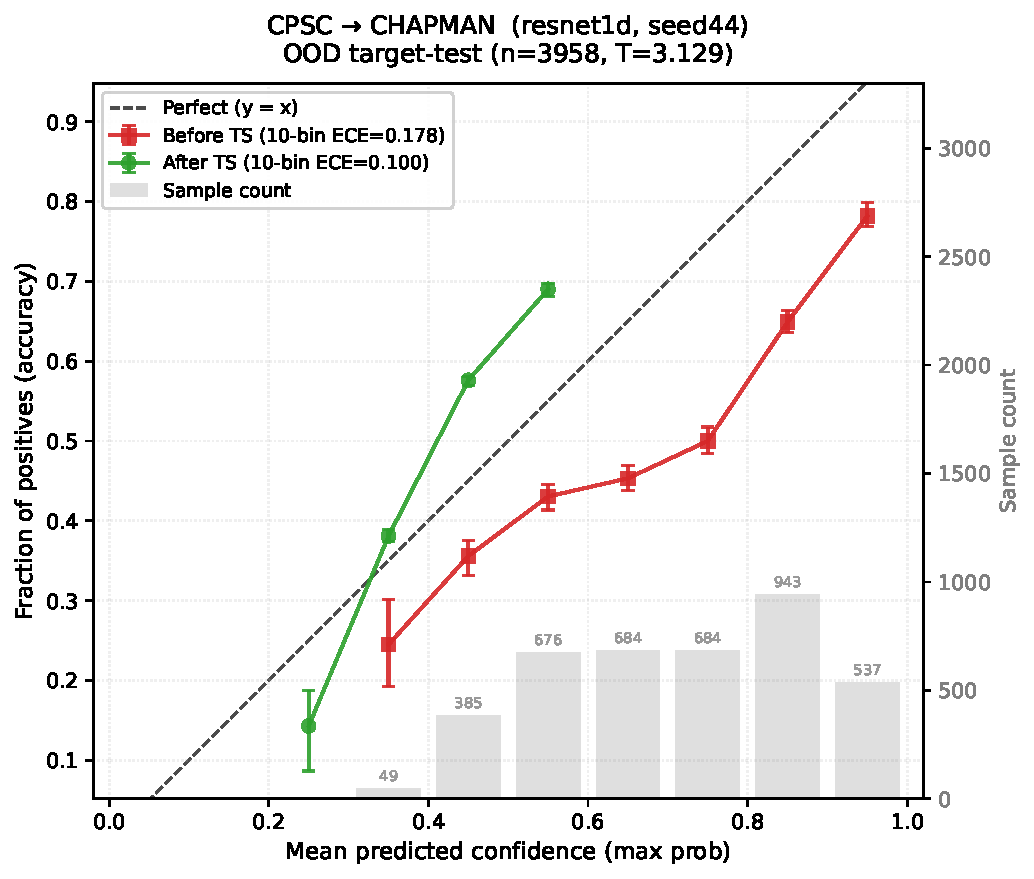
\includegraphics[width=0.32\textwidth]{figures/fig_reliability_supp_cpsc_chapman_resnet1d_seed44.pdf}
\caption{CPSC$\to$Chapman reliability diagrams: ResNet1D seeds 42--44.}
\end{figure}

\begin{figure}[h]
\centering
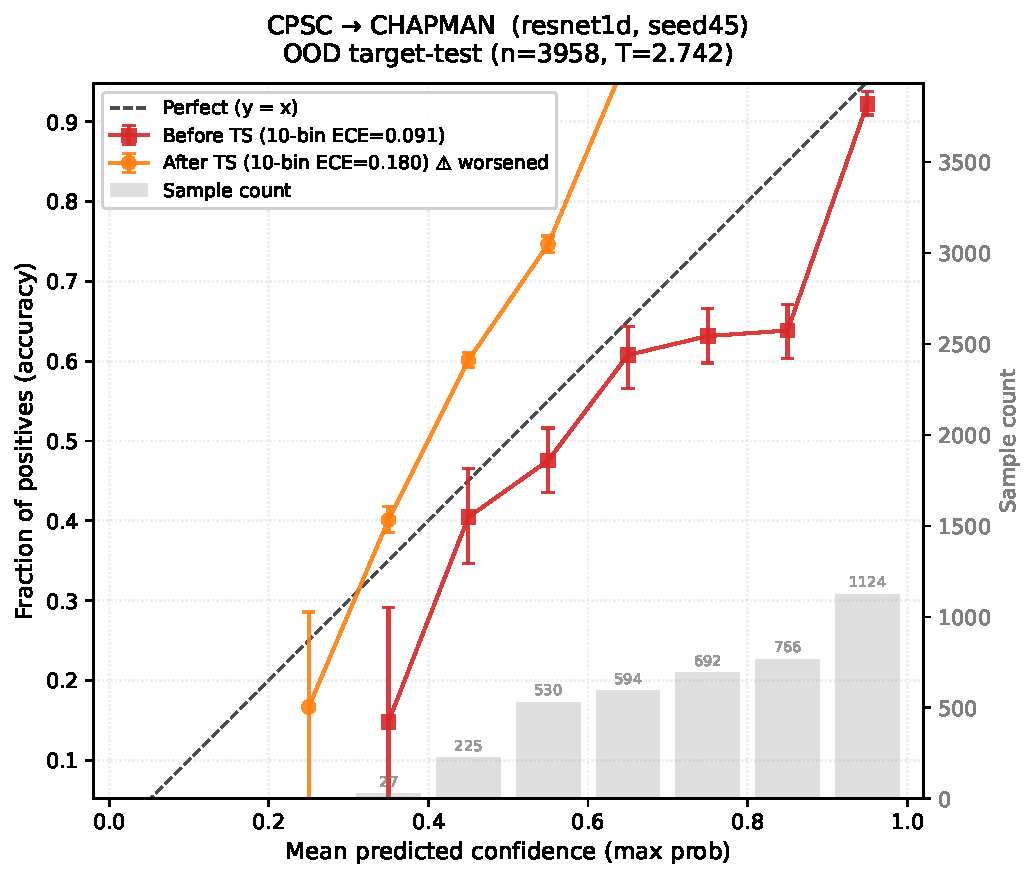
\includegraphics[width=0.45\textwidth]{figures/fig_reliability_supp_cpsc_chapman_resnet1d_seed45.pdf}
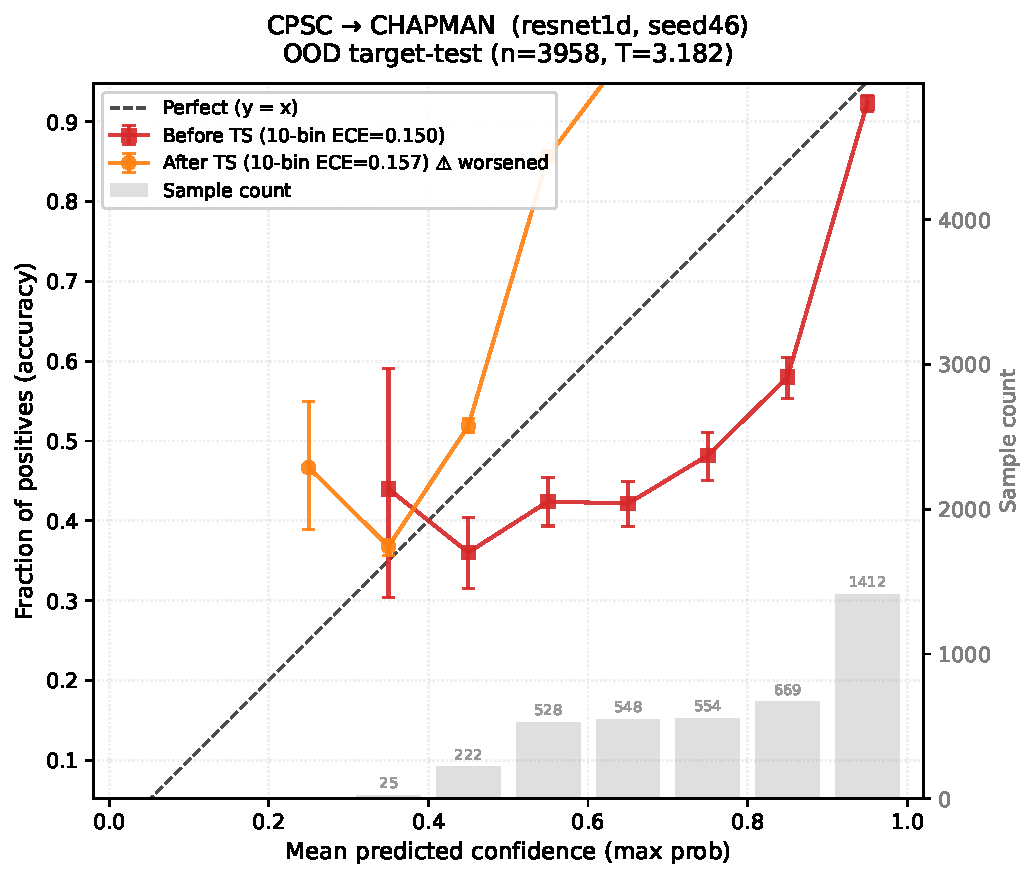
\includegraphics[width=0.45\textwidth]{figures/fig_reliability_supp_cpsc_chapman_resnet1d_seed46.pdf}
\caption{CPSC$\to$Chapman reliability diagrams: ResNet1D seeds 45--46.}
\end{figure}

\begin{figure}[h]
\centering
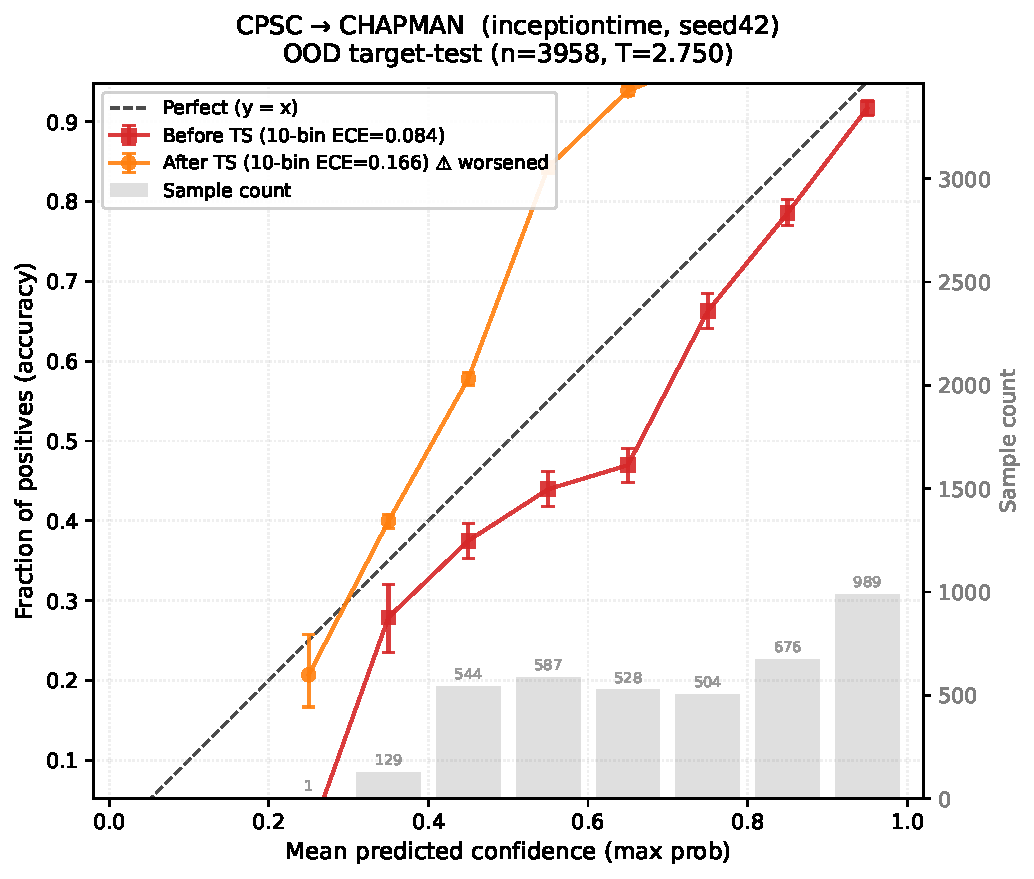
\includegraphics[width=0.32\textwidth]{figures/fig_reliability_supp_cpsc_chapman_inceptiontime_seed42.pdf}
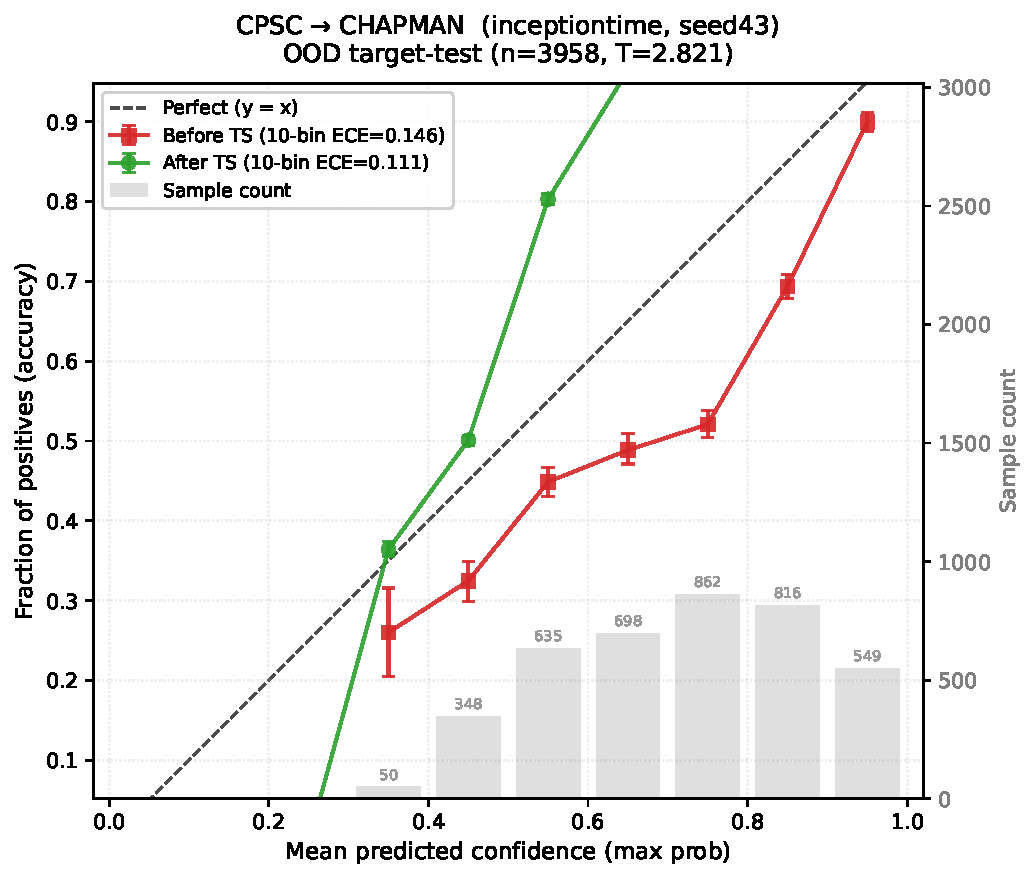
\includegraphics[width=0.32\textwidth]{figures/fig_reliability_supp_cpsc_chapman_inceptiontime_seed43.pdf}
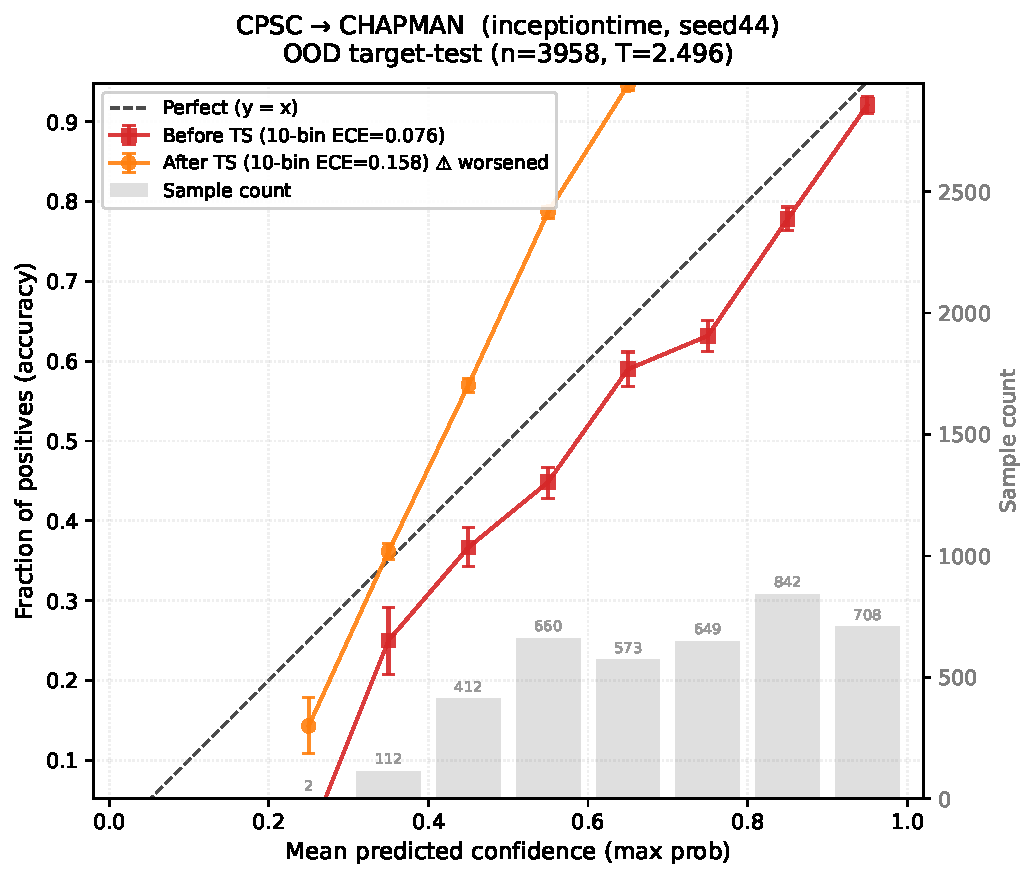
\includegraphics[width=0.32\textwidth]{figures/fig_reliability_supp_cpsc_chapman_inceptiontime_seed44.pdf}
\caption{CPSC$\to$Chapman reliability diagrams: InceptionTime seeds 42--44.}
\end{figure}

\begin{figure}[h]
\centering
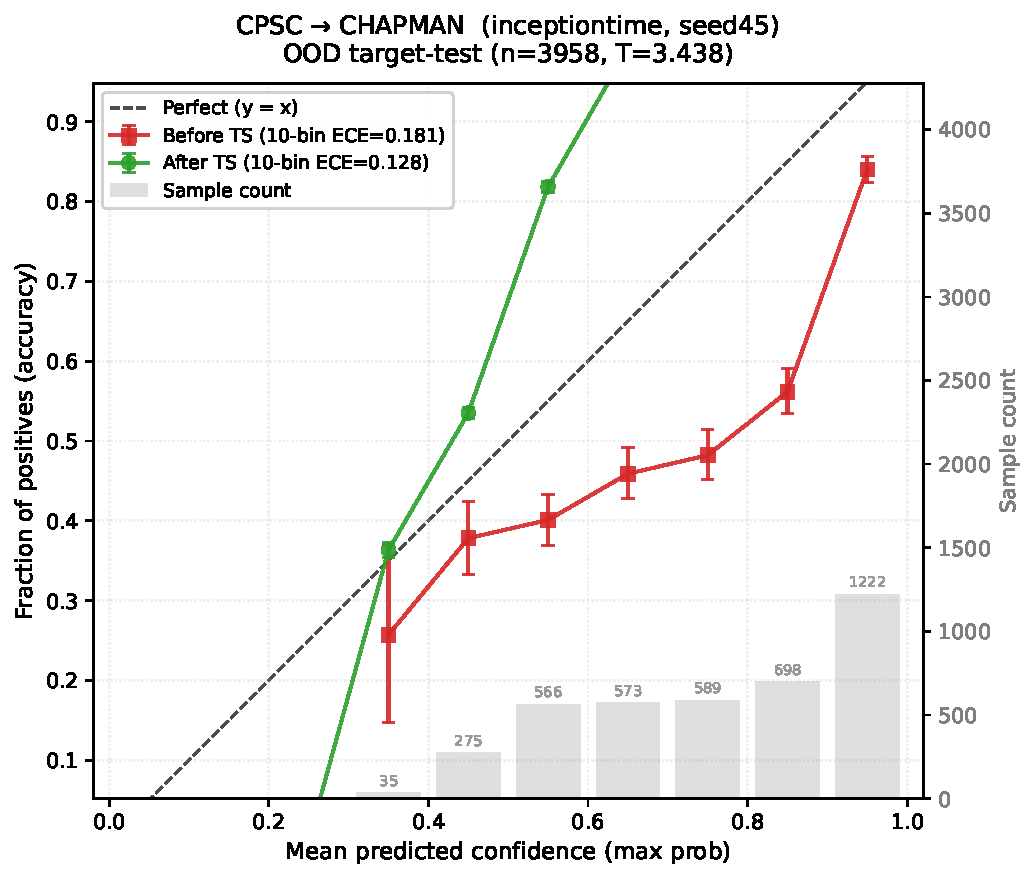
\includegraphics[width=0.45\textwidth]{figures/fig_reliability_supp_cpsc_chapman_inceptiontime_seed45.pdf}
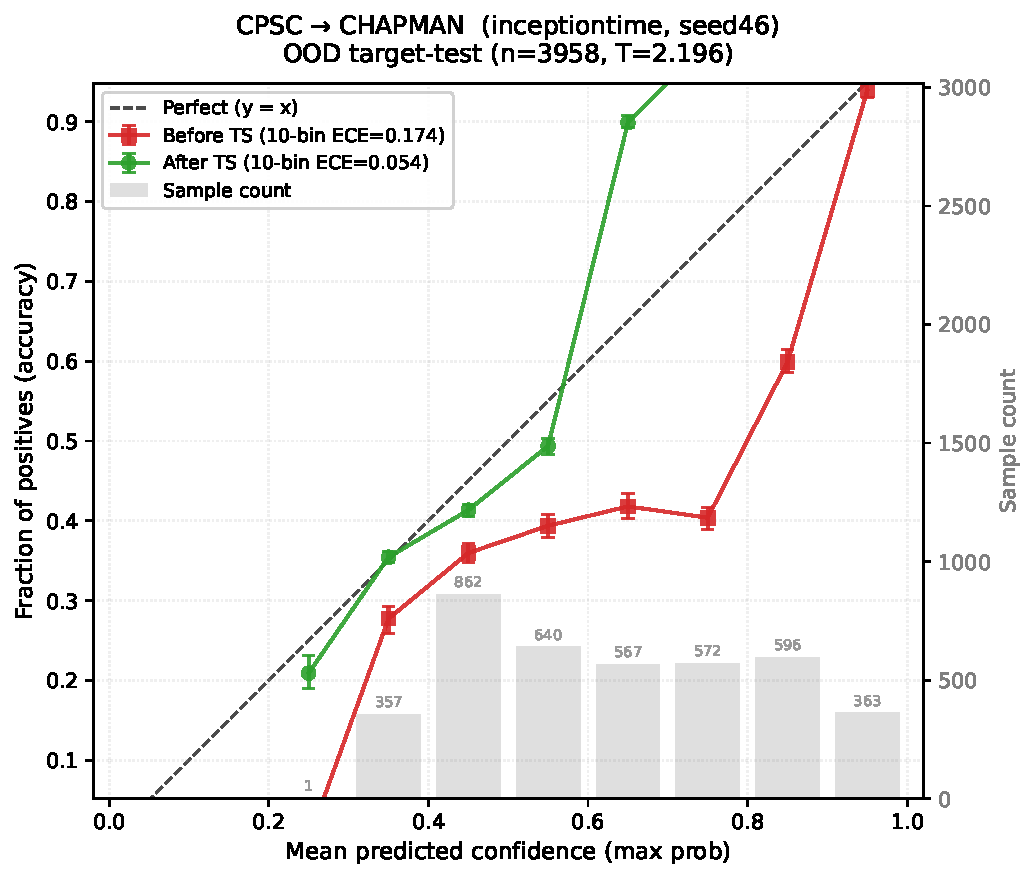
\includegraphics[width=0.45\textwidth]{figures/fig_reliability_supp_cpsc_chapman_inceptiontime_seed46.pdf}
\caption{CPSC$\to$Chapman reliability diagrams: InceptionTime seeds 45--46.}
\end{figure}

\subsubsection*{S1.4.\ CPSC$\rightarrow$PTB-XL}

\begin{figure}[h]
\centering
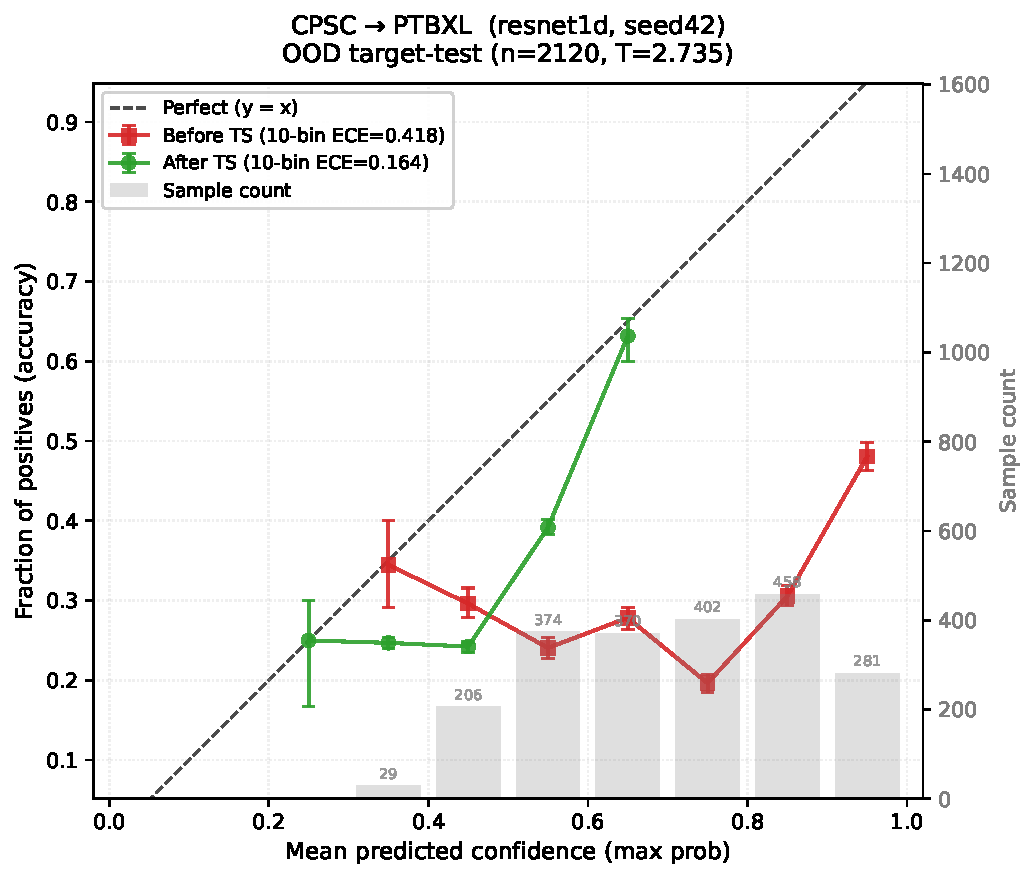
\includegraphics[width=0.32\textwidth]{figures/fig_reliability_supp_cpsc_ptbxl_resnet1d_seed42.pdf}
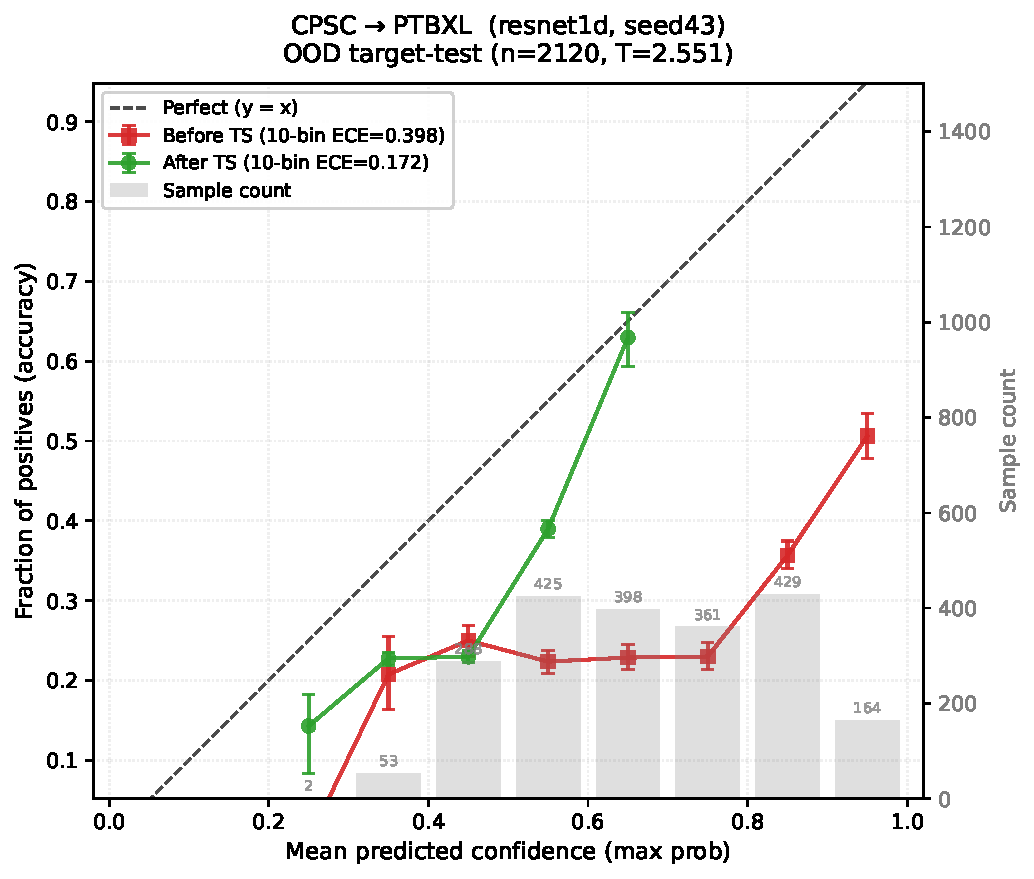
\includegraphics[width=0.32\textwidth]{figures/fig_reliability_supp_cpsc_ptbxl_resnet1d_seed43.pdf}
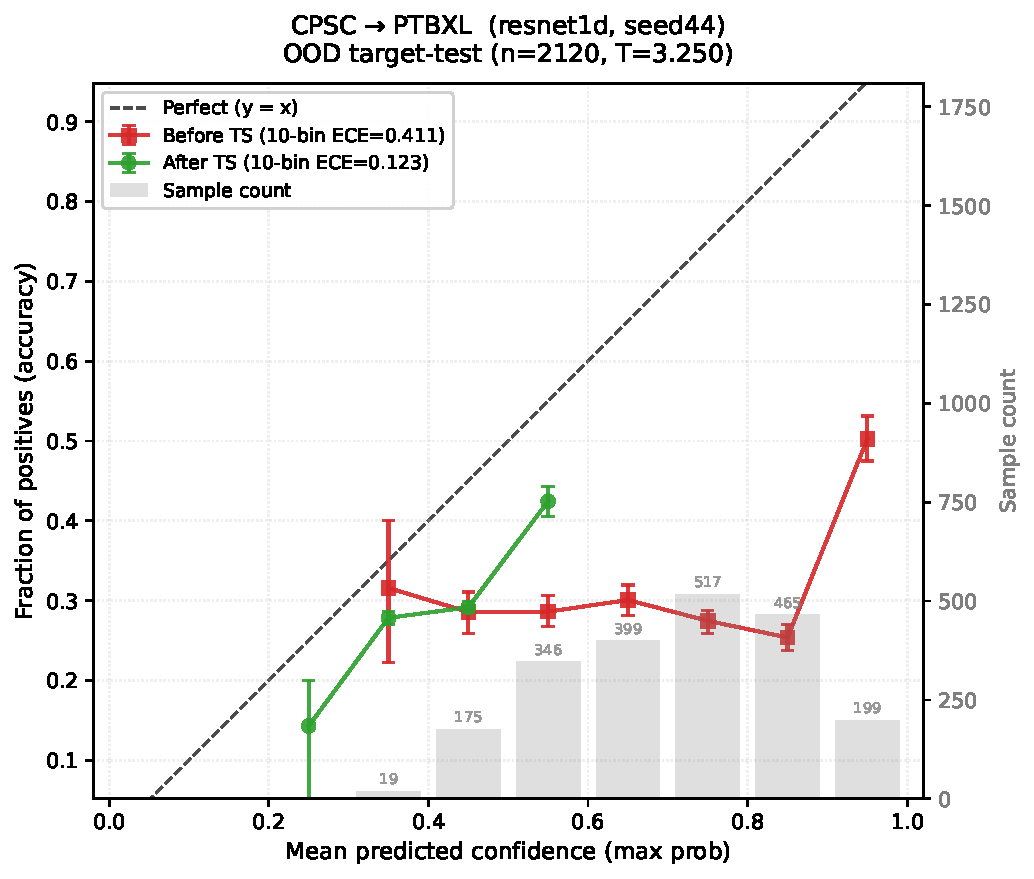
\includegraphics[width=0.32\textwidth]{figures/fig_reliability_supp_cpsc_ptbxl_resnet1d_seed44.pdf}
\caption{CPSC$\to$PTB-XL reliability diagrams: ResNet1D seeds 42--44.}
\end{figure}

\begin{figure}[h]
\centering
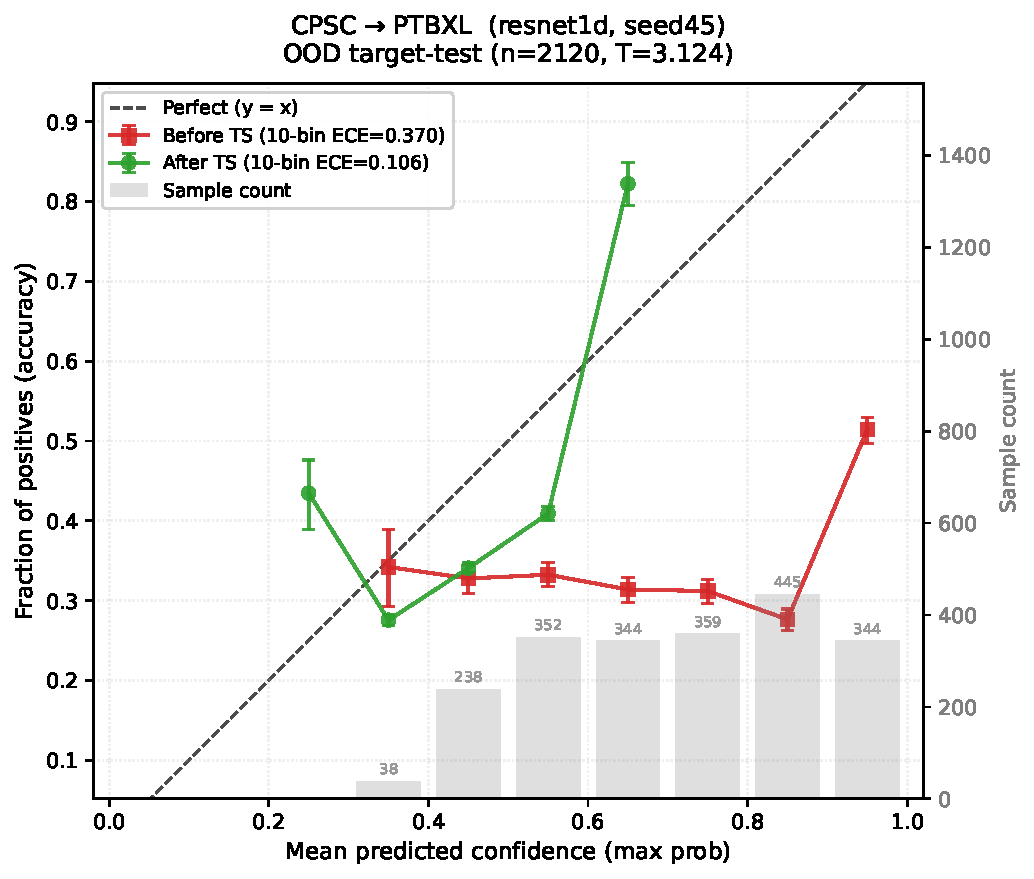
\includegraphics[width=0.45\textwidth]{figures/fig_reliability_supp_cpsc_ptbxl_resnet1d_seed45.pdf}
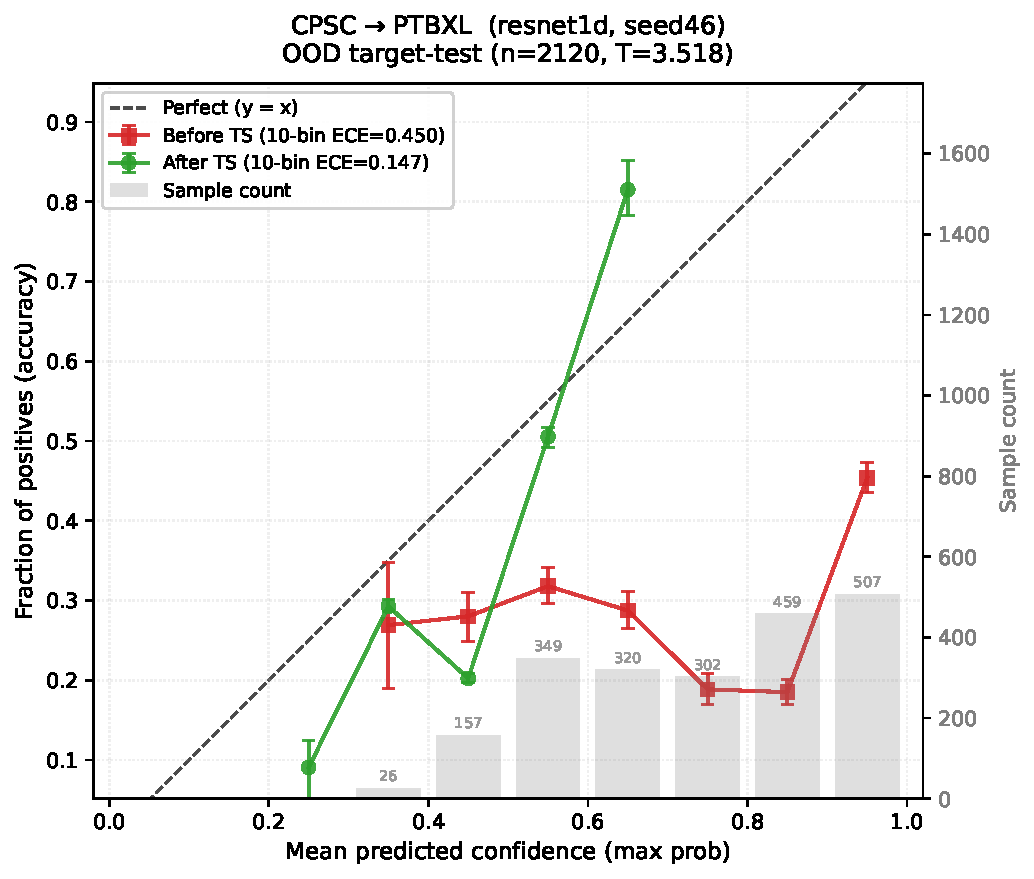
\includegraphics[width=0.45\textwidth]{figures/fig_reliability_supp_cpsc_ptbxl_resnet1d_seed46.pdf}
\caption{CPSC$\to$PTB-XL reliability diagrams: ResNet1D seeds 45--46.}
\end{figure}

\begin{figure}[h]
\centering
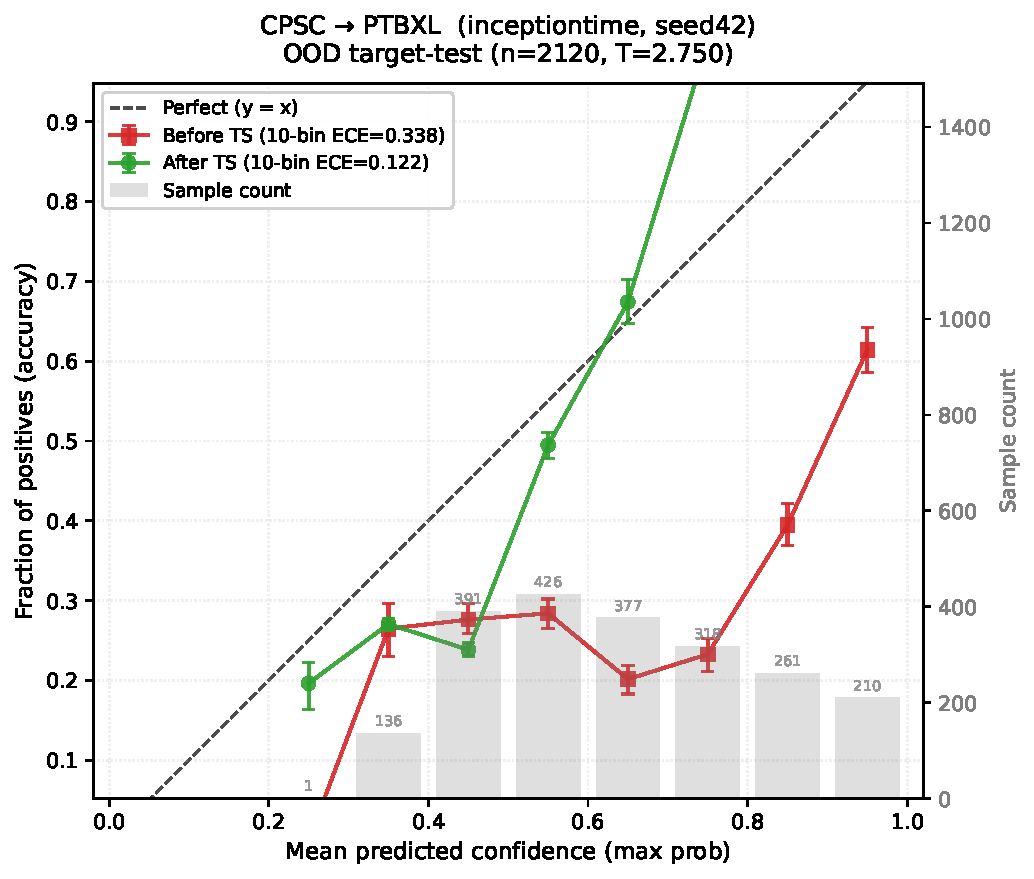
\includegraphics[width=0.32\textwidth]{figures/fig_reliability_supp_cpsc_ptbxl_inceptiontime_seed42.pdf}
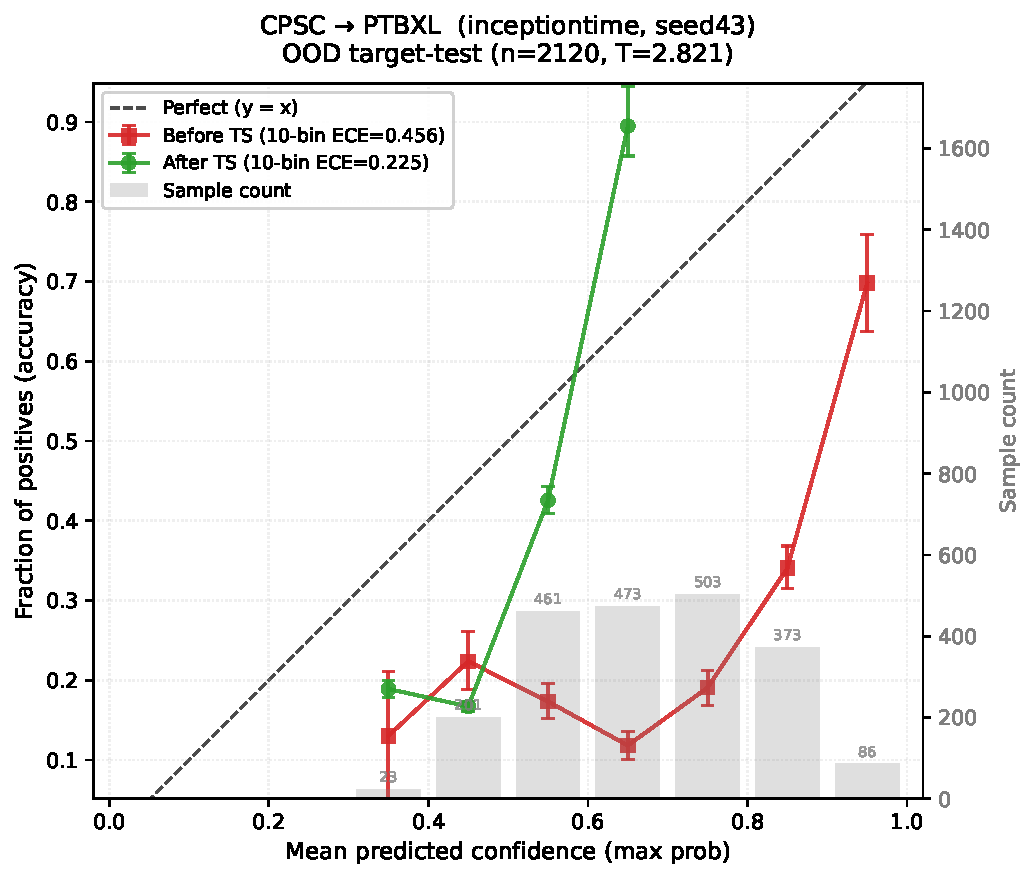
\includegraphics[width=0.32\textwidth]{figures/fig_reliability_supp_cpsc_ptbxl_inceptiontime_seed43.pdf}
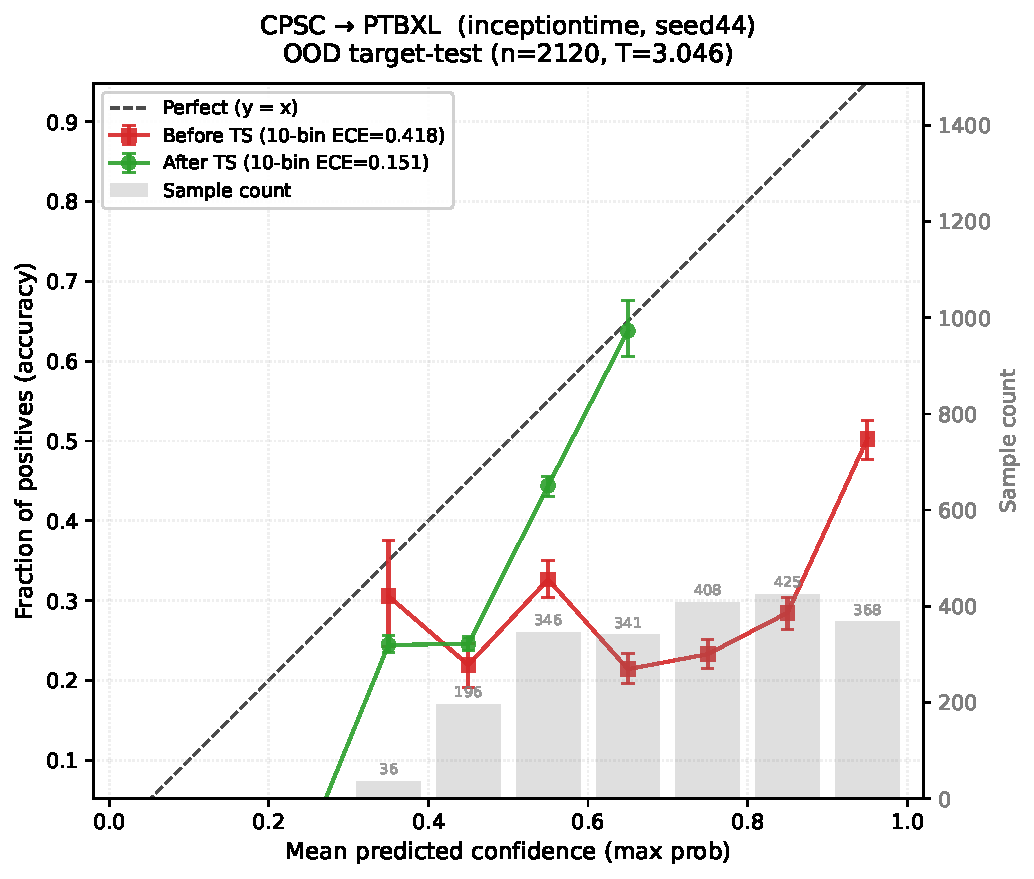
\includegraphics[width=0.32\textwidth]{figures/fig_reliability_supp_cpsc_ptbxl_inceptiontime_seed44.pdf}
\caption{CPSC$\to$PTB-XL reliability diagrams: InceptionTime seeds 42--44.}
\end{figure}

\begin{figure}[h]
\centering
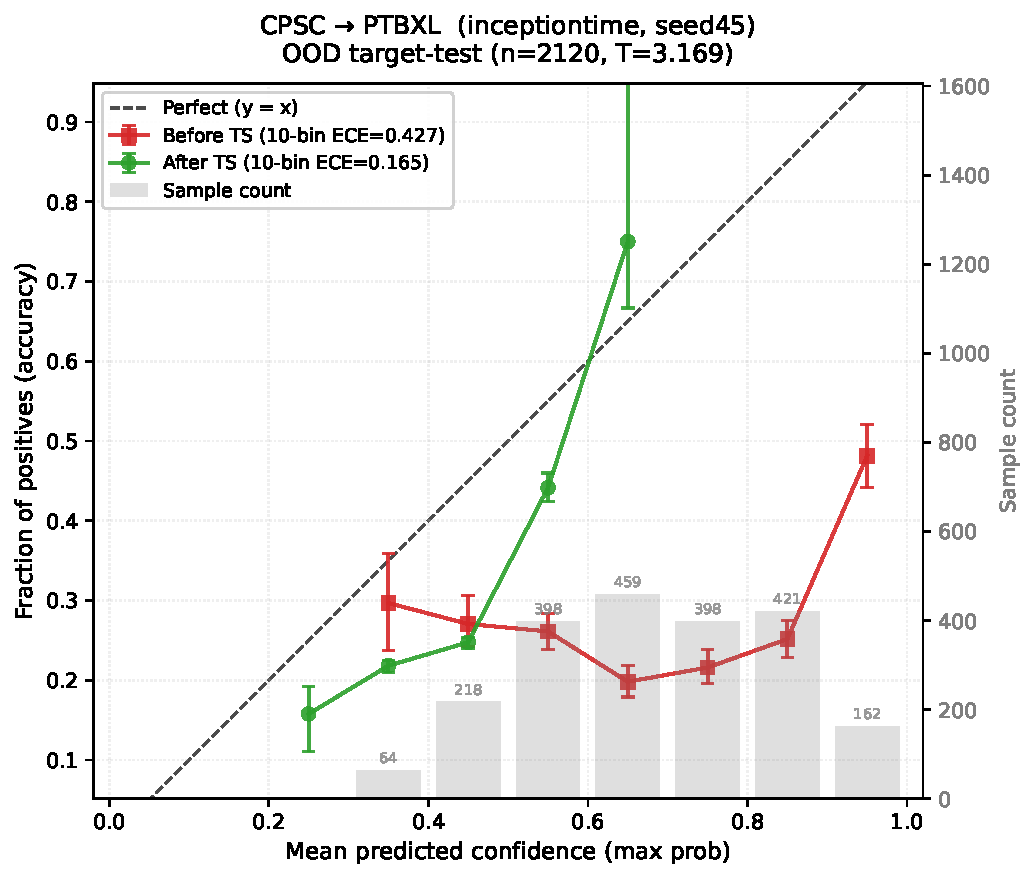
\includegraphics[width=0.45\textwidth]{figures/fig_reliability_supp_cpsc_ptbxl_inceptiontime_seed45.pdf}
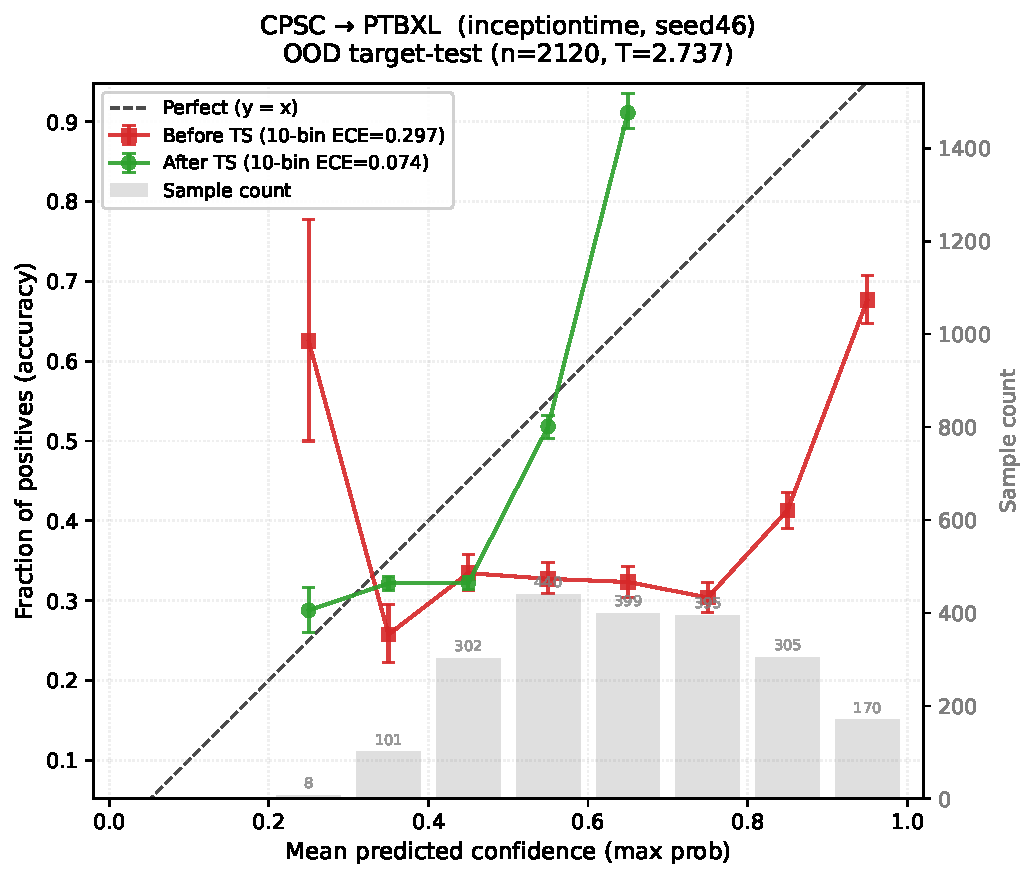
\includegraphics[width=0.45\textwidth]{figures/fig_reliability_supp_cpsc_ptbxl_inceptiontime_seed46.pdf}
\caption{CPSC$\to$PTB-XL reliability diagrams: InceptionTime seeds 45--46.}
\end{figure}

\subsubsection*{S1.5.\ PTB-XL$\rightarrow$Chapman}

\begin{figure}[h]
\centering
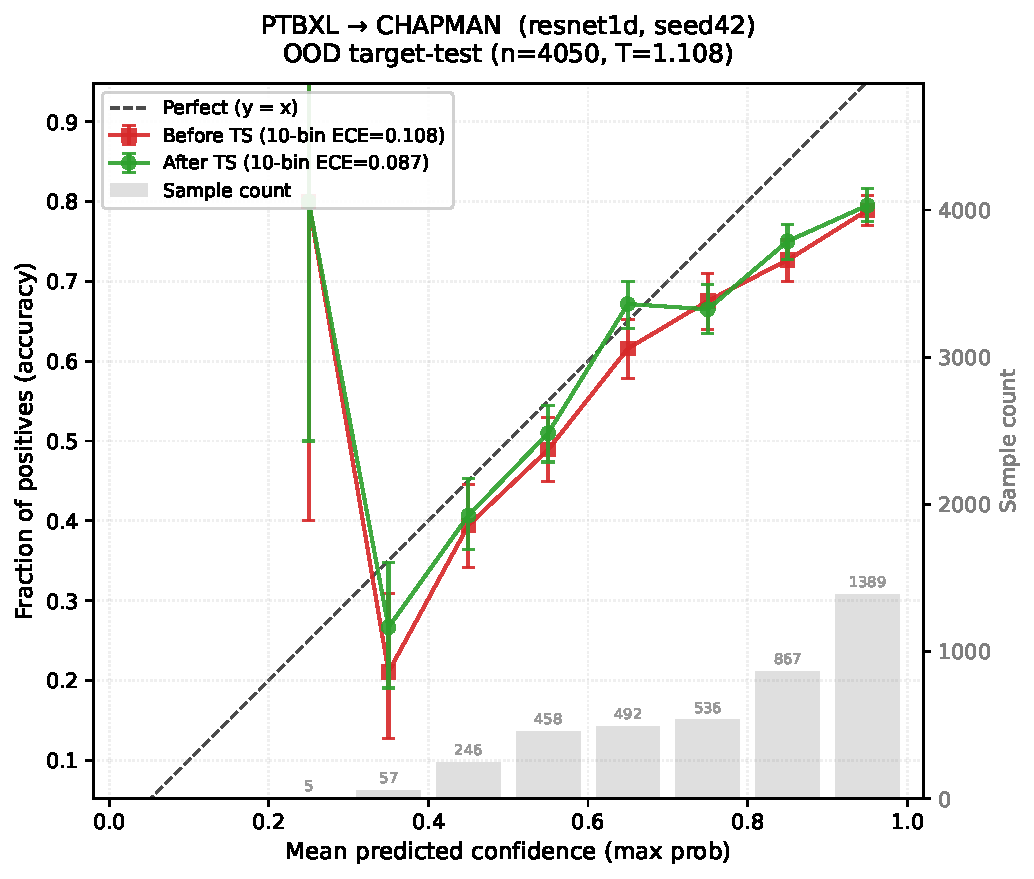
\includegraphics[width=0.32\textwidth]{figures/fig_reliability_supp_ptbxl_chapman_resnet1d_seed42.pdf}
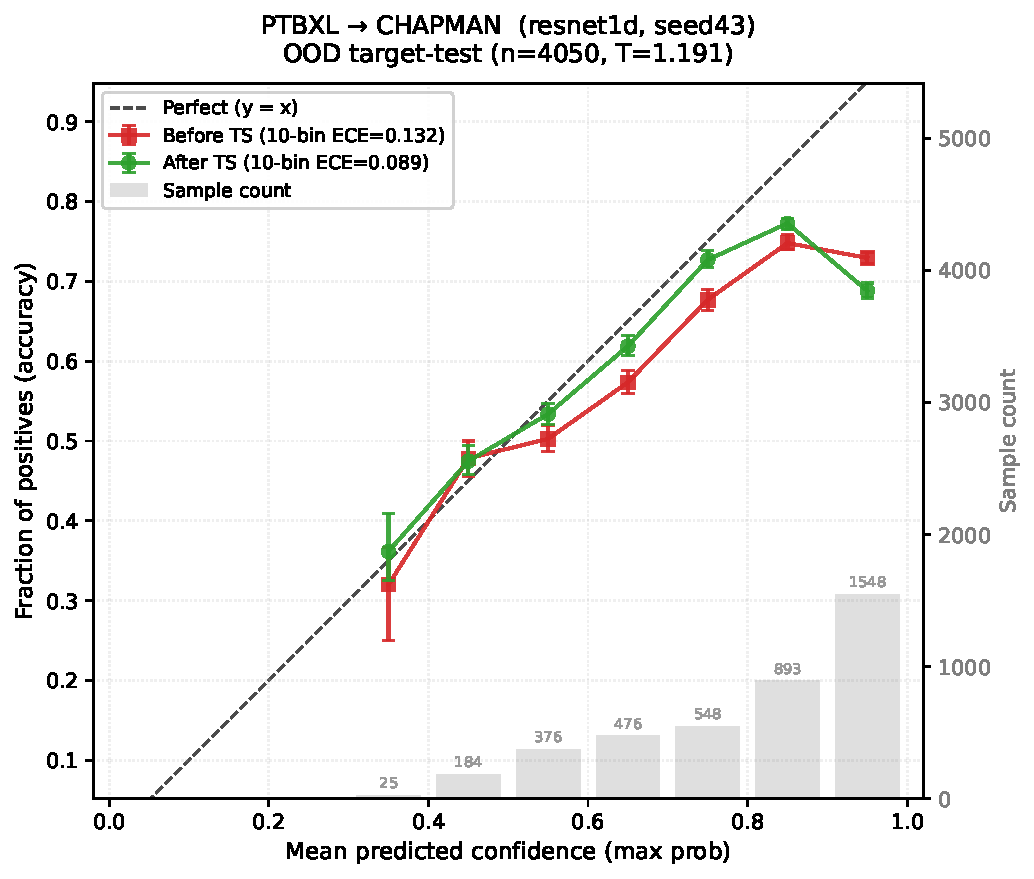
\includegraphics[width=0.32\textwidth]{figures/fig_reliability_supp_ptbxl_chapman_resnet1d_seed43.pdf}
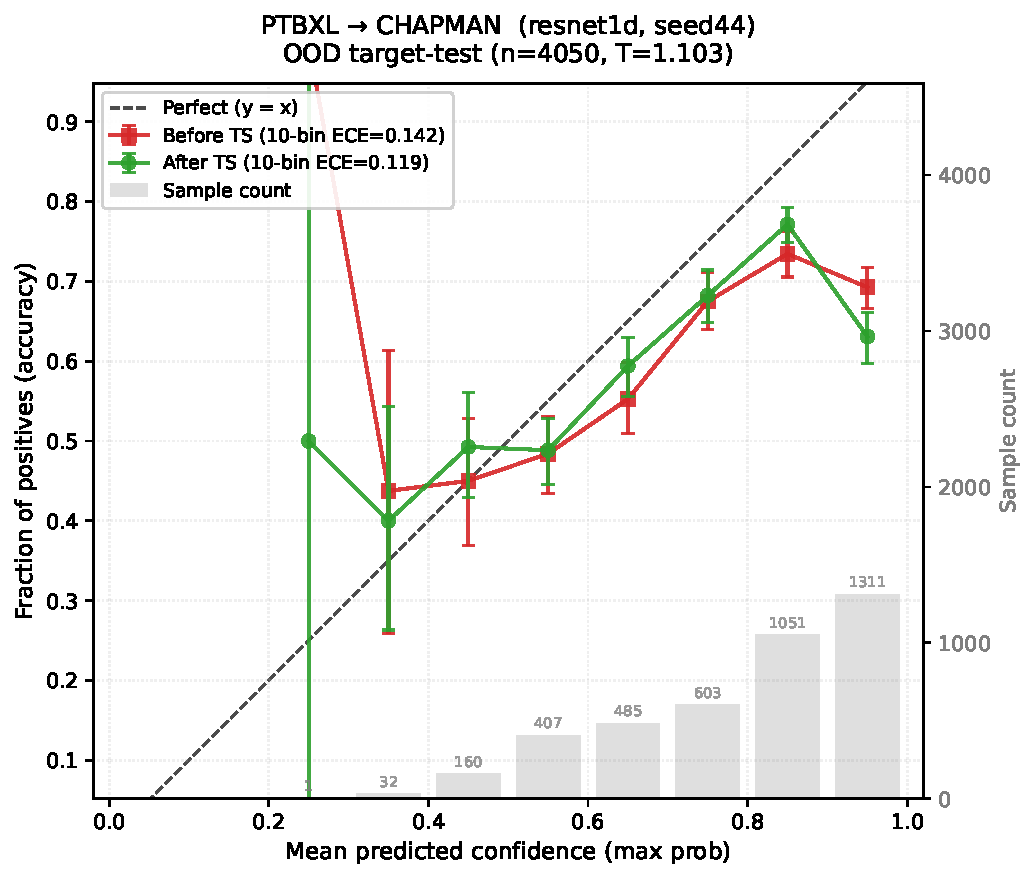
\includegraphics[width=0.32\textwidth]{figures/fig_reliability_supp_ptbxl_chapman_resnet1d_seed44.pdf}
\caption{PTB-XL$\to$Chapman reliability diagrams: ResNet1D seeds 42--44.}
\end{figure}

\begin{figure}[h]
\centering
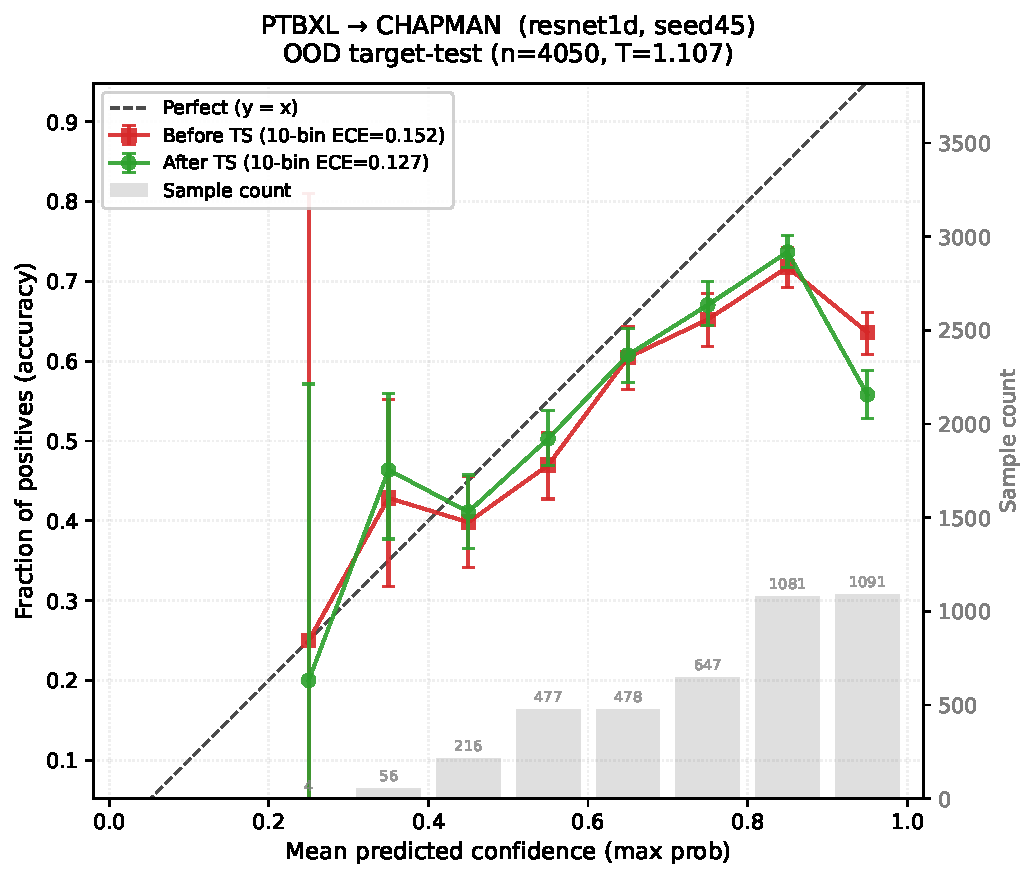
\includegraphics[width=0.45\textwidth]{figures/fig_reliability_supp_ptbxl_chapman_resnet1d_seed45.pdf}
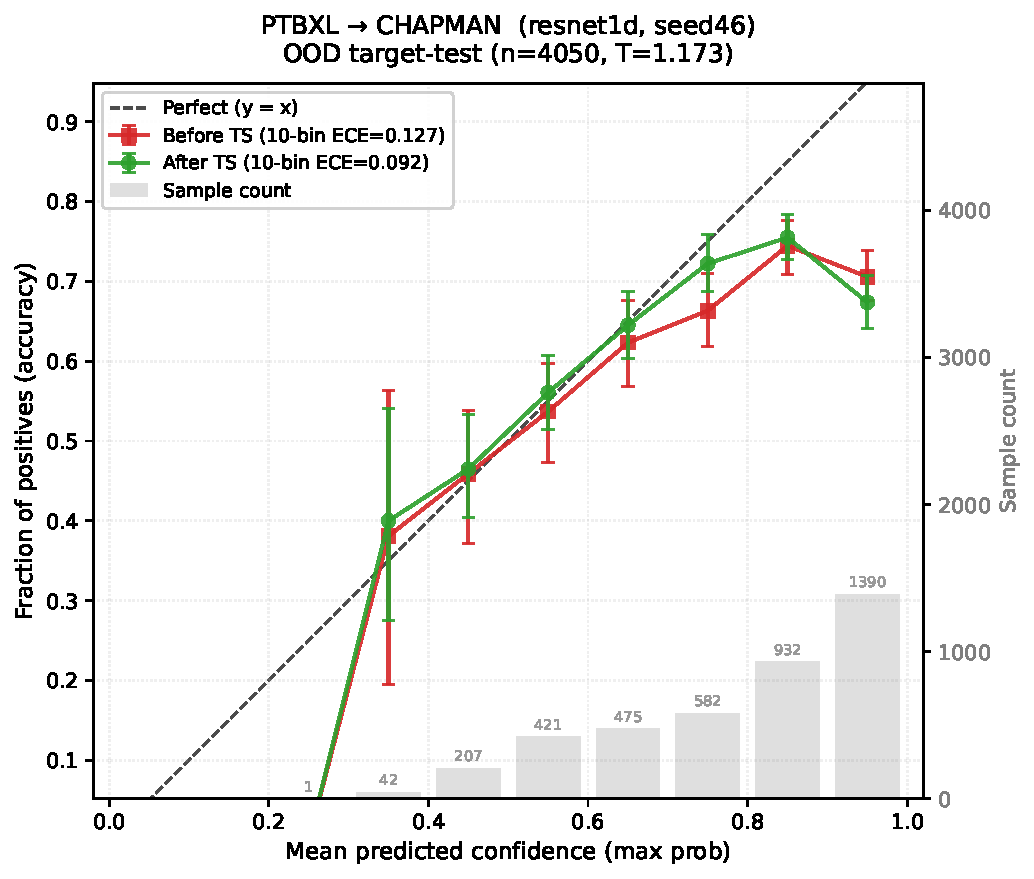
\includegraphics[width=0.45\textwidth]{figures/fig_reliability_supp_ptbxl_chapman_resnet1d_seed46.pdf}
\caption{PTB-XL$\to$Chapman reliability diagrams: ResNet1D seeds 45--46.}
\end{figure}

\begin{figure}[h]
\centering
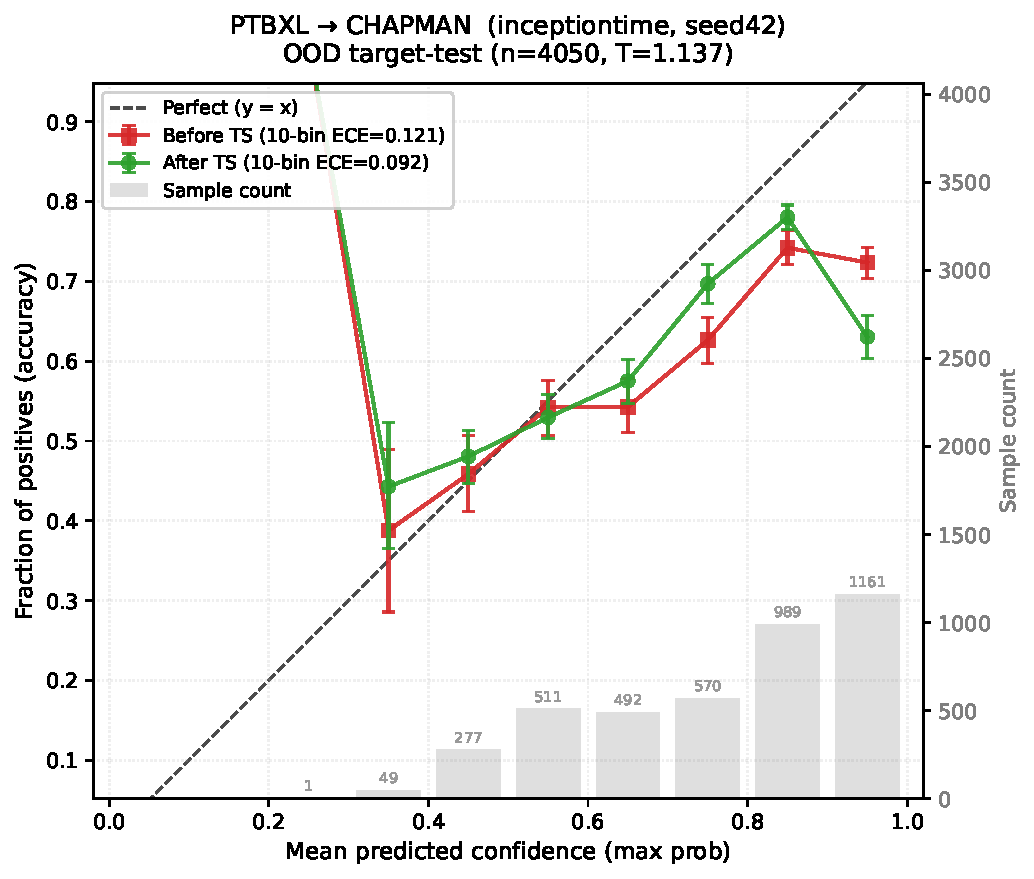
\includegraphics[width=0.32\textwidth]{figures/fig_reliability_supp_ptbxl_chapman_inceptiontime_seed42.pdf}
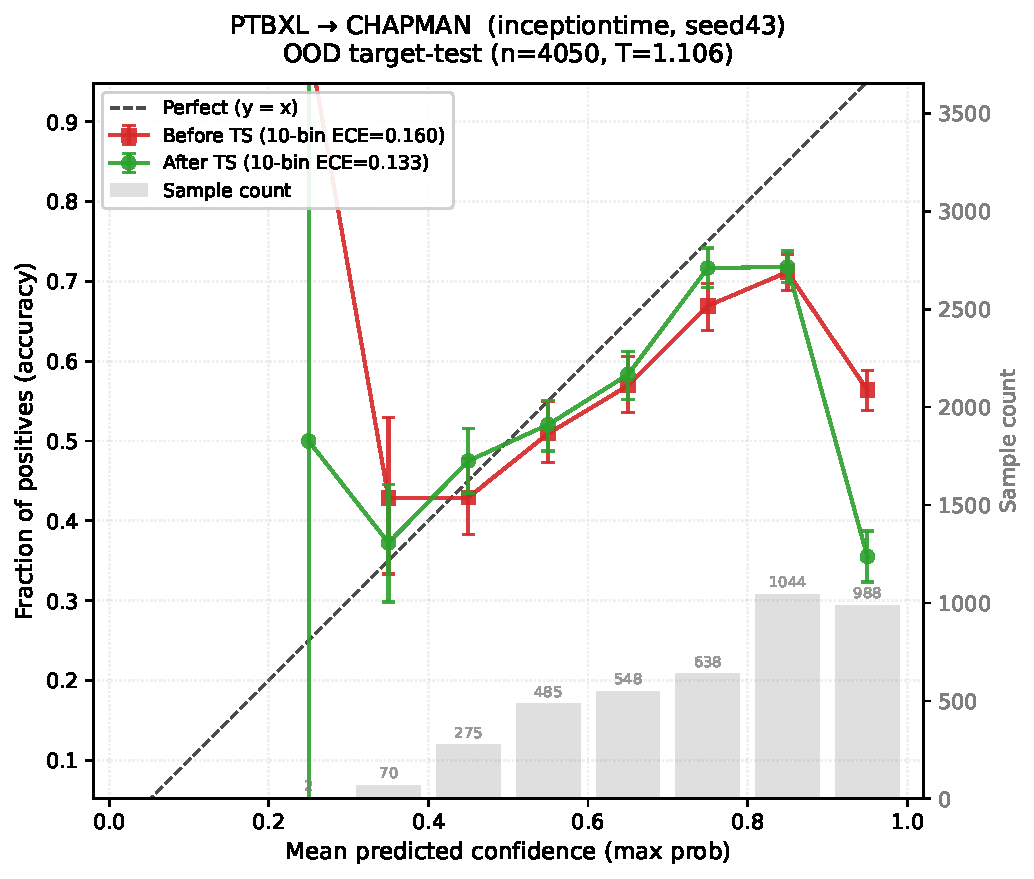
\includegraphics[width=0.32\textwidth]{figures/fig_reliability_supp_ptbxl_chapman_inceptiontime_seed43.pdf}
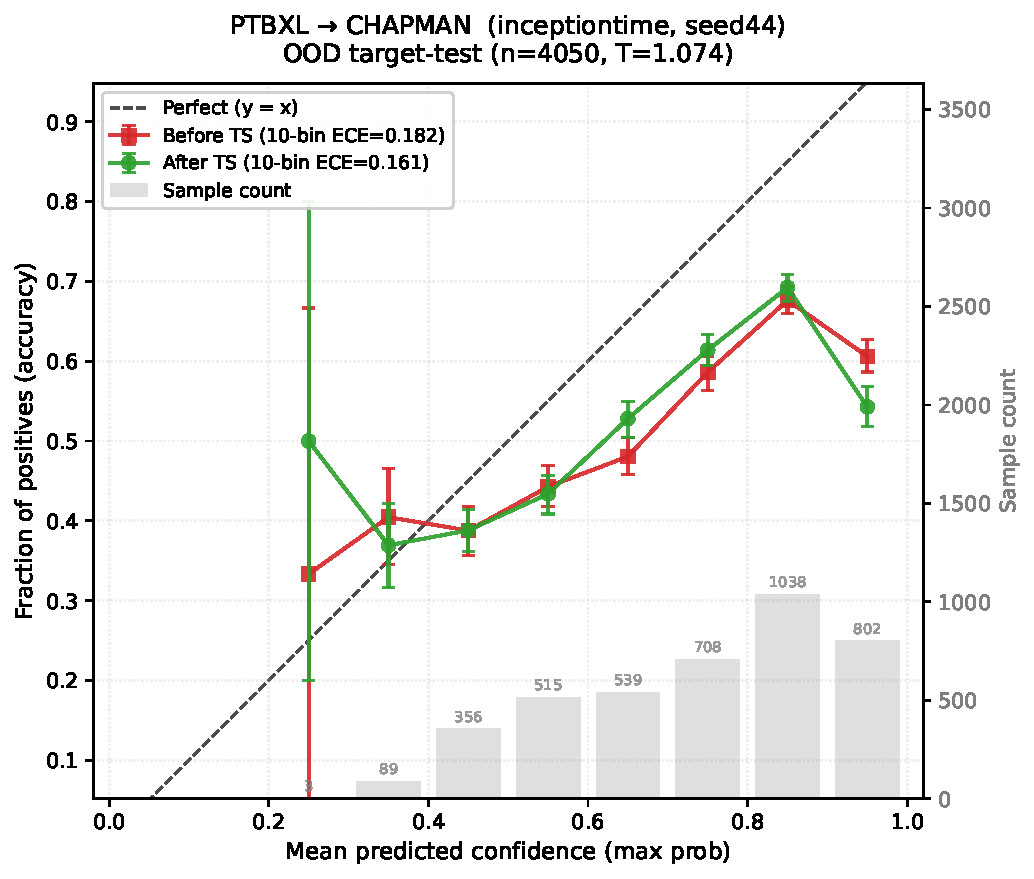
\includegraphics[width=0.32\textwidth]{figures/fig_reliability_supp_ptbxl_chapman_inceptiontime_seed44.pdf}
\caption{PTB-XL$\to$Chapman reliability diagrams: InceptionTime seeds 42--44.}
\end{figure}

\begin{figure}[h]
\centering
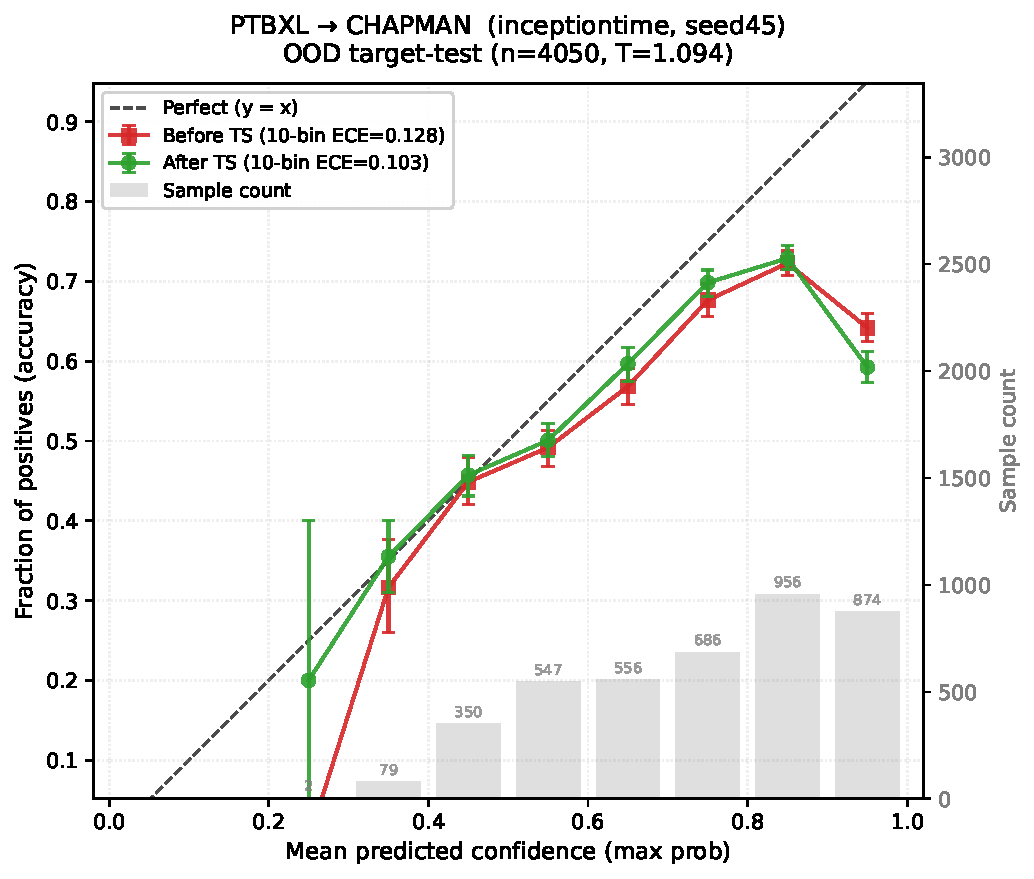
\includegraphics[width=0.45\textwidth]{figures/fig_reliability_supp_ptbxl_chapman_inceptiontime_seed45.pdf}
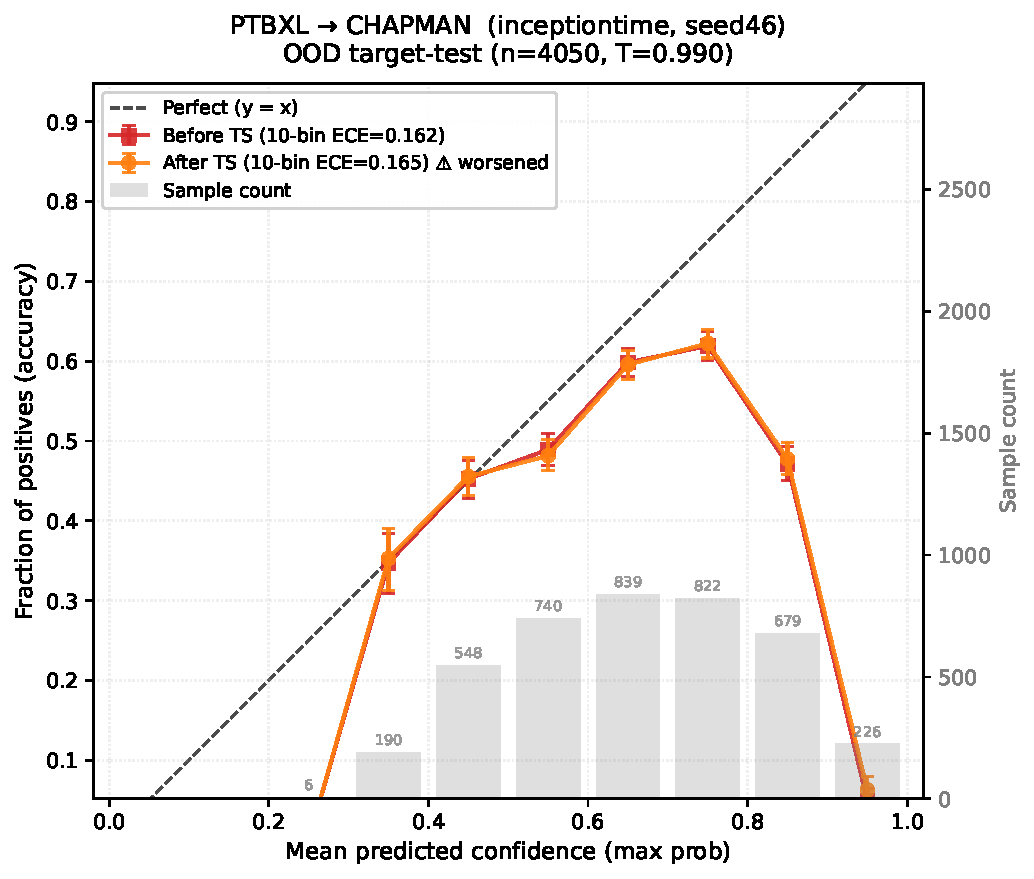
\includegraphics[width=0.45\textwidth]{figures/fig_reliability_supp_ptbxl_chapman_inceptiontime_seed46.pdf}
\caption{PTB-XL$\to$Chapman reliability diagrams: InceptionTime seeds 45--46.}
\end{figure}

\subsubsection*{S1.6.\ PTB-XL$\rightarrow$CPSC}

\begin{figure}[h]
\centering
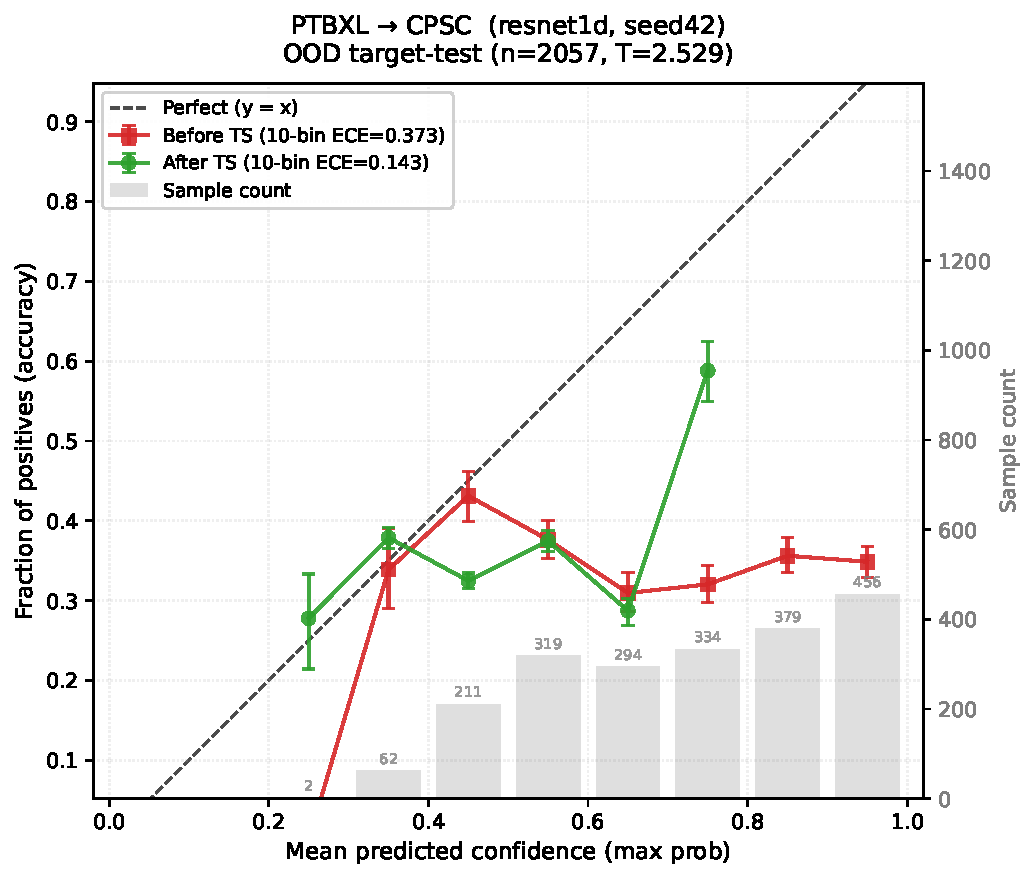
\includegraphics[width=0.32\textwidth]{figures/fig_reliability_supp_ptbxl_cpsc_resnet1d_seed42.pdf}
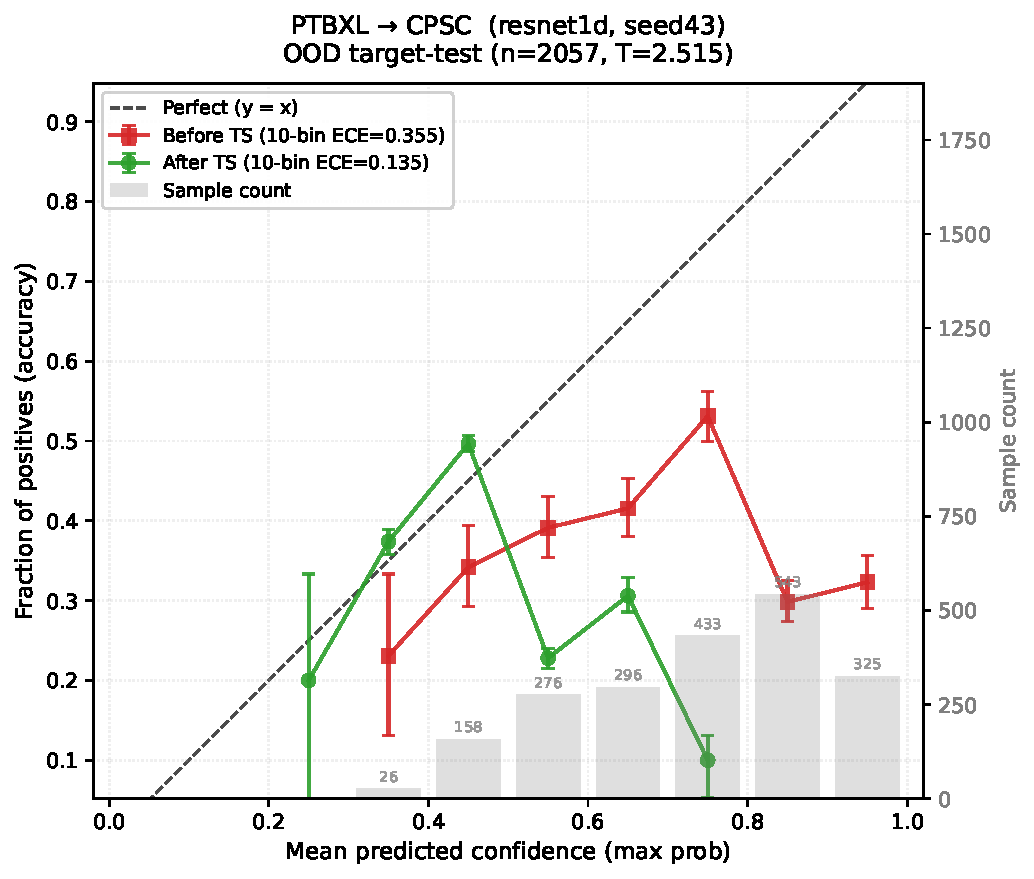
\includegraphics[width=0.32\textwidth]{figures/fig_reliability_supp_ptbxl_cpsc_resnet1d_seed43.pdf}
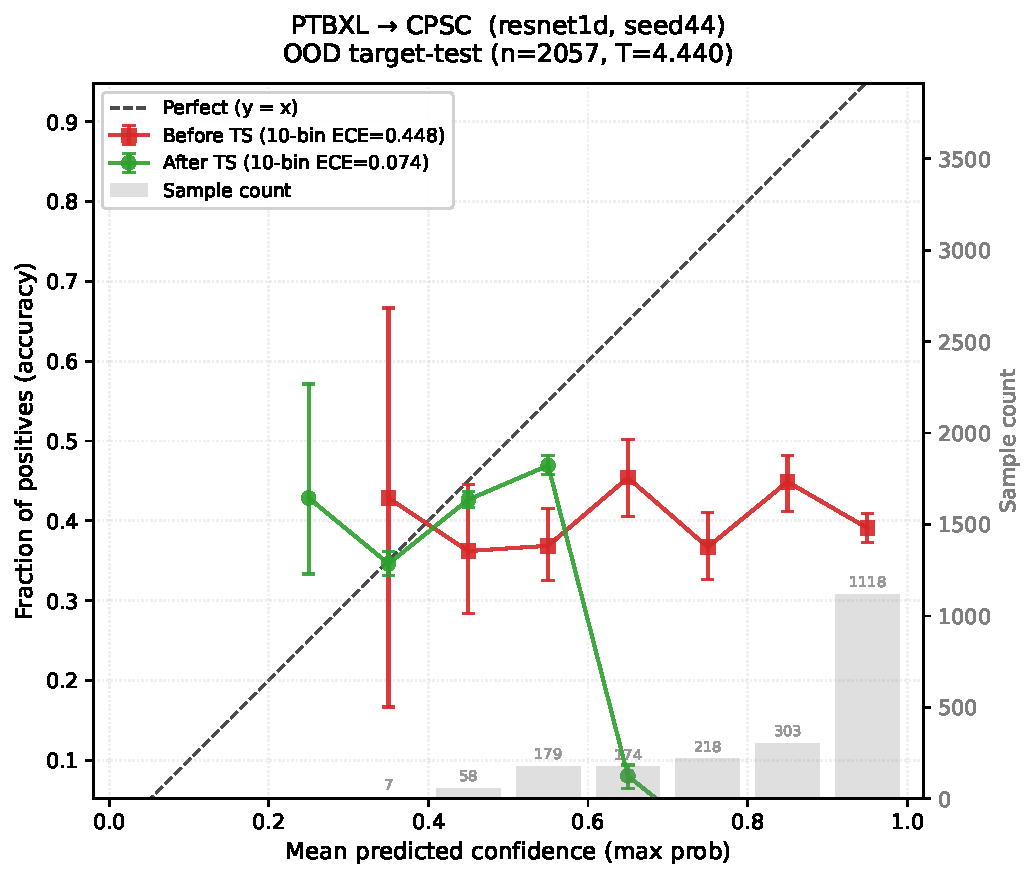
\includegraphics[width=0.32\textwidth]{figures/fig_reliability_supp_ptbxl_cpsc_resnet1d_seed44.pdf}
\caption{PTB-XL$\to$CPSC reliability diagrams: ResNet1D seeds 42--44.}
\end{figure}

\begin{figure}[h]
\centering
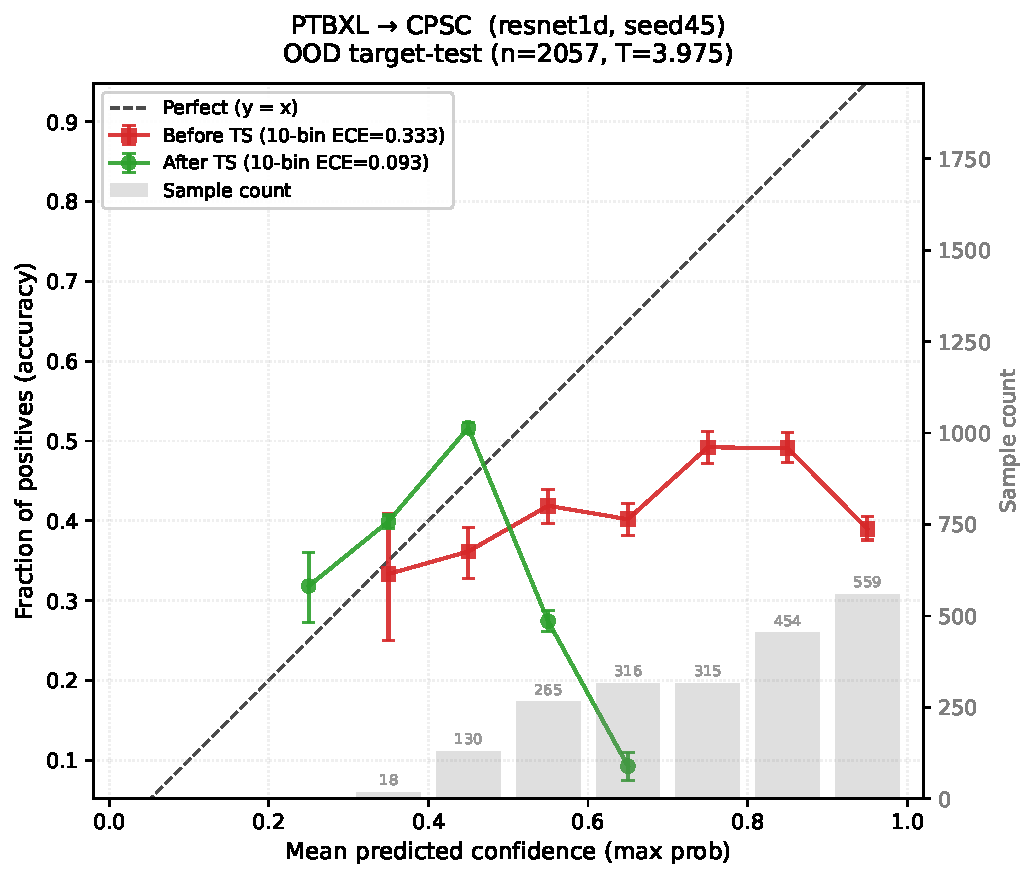
\includegraphics[width=0.45\textwidth]{figures/fig_reliability_supp_ptbxl_cpsc_resnet1d_seed45.pdf}
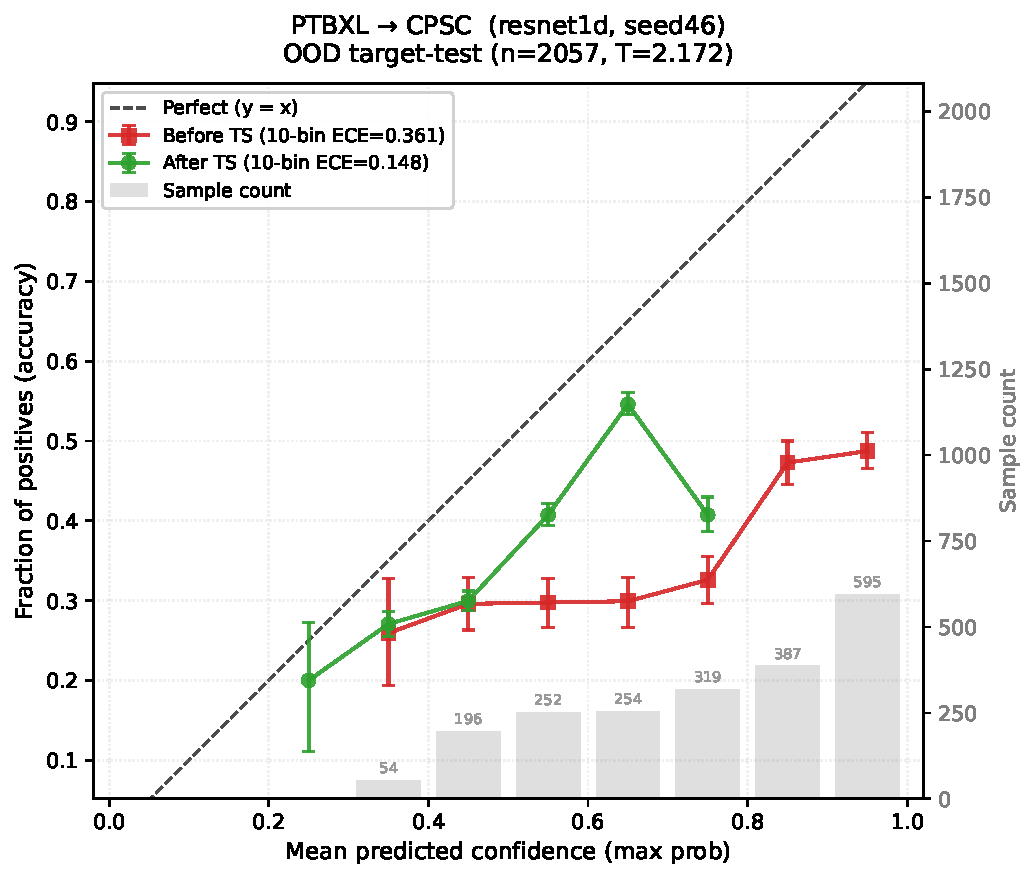
\includegraphics[width=0.45\textwidth]{figures/fig_reliability_supp_ptbxl_cpsc_resnet1d_seed46.pdf}
\caption{PTB-XL$\to$CPSC reliability diagrams: ResNet1D seeds 45--46.}
\end{figure}

\begin{figure}[h]
\centering
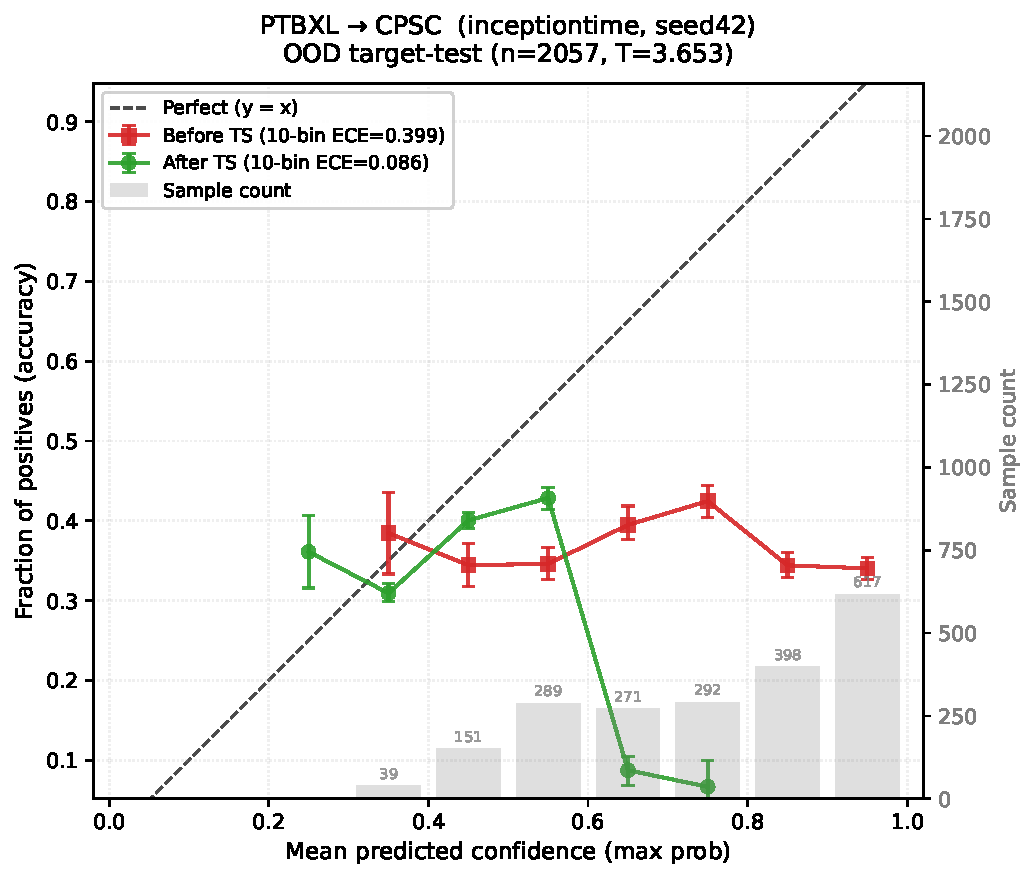
\includegraphics[width=0.32\textwidth]{figures/fig_reliability_supp_ptbxl_cpsc_inceptiontime_seed42.pdf}
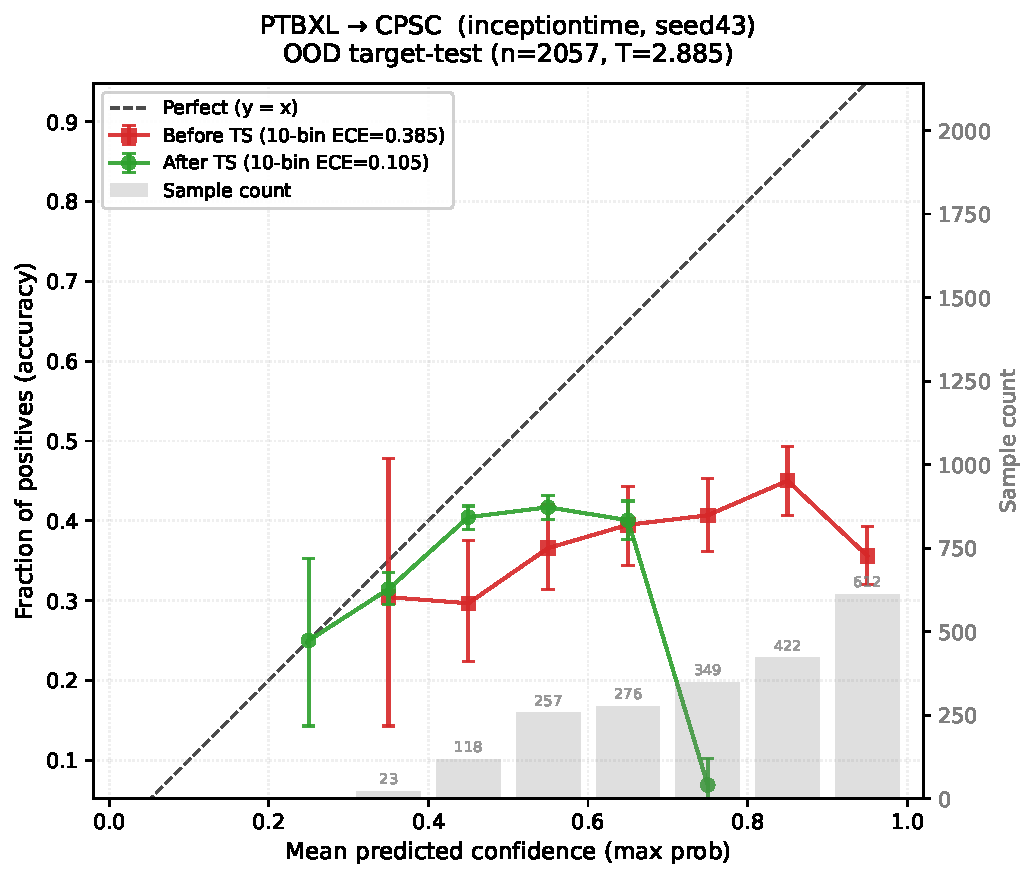
\includegraphics[width=0.32\textwidth]{figures/fig_reliability_supp_ptbxl_cpsc_inceptiontime_seed43.pdf}
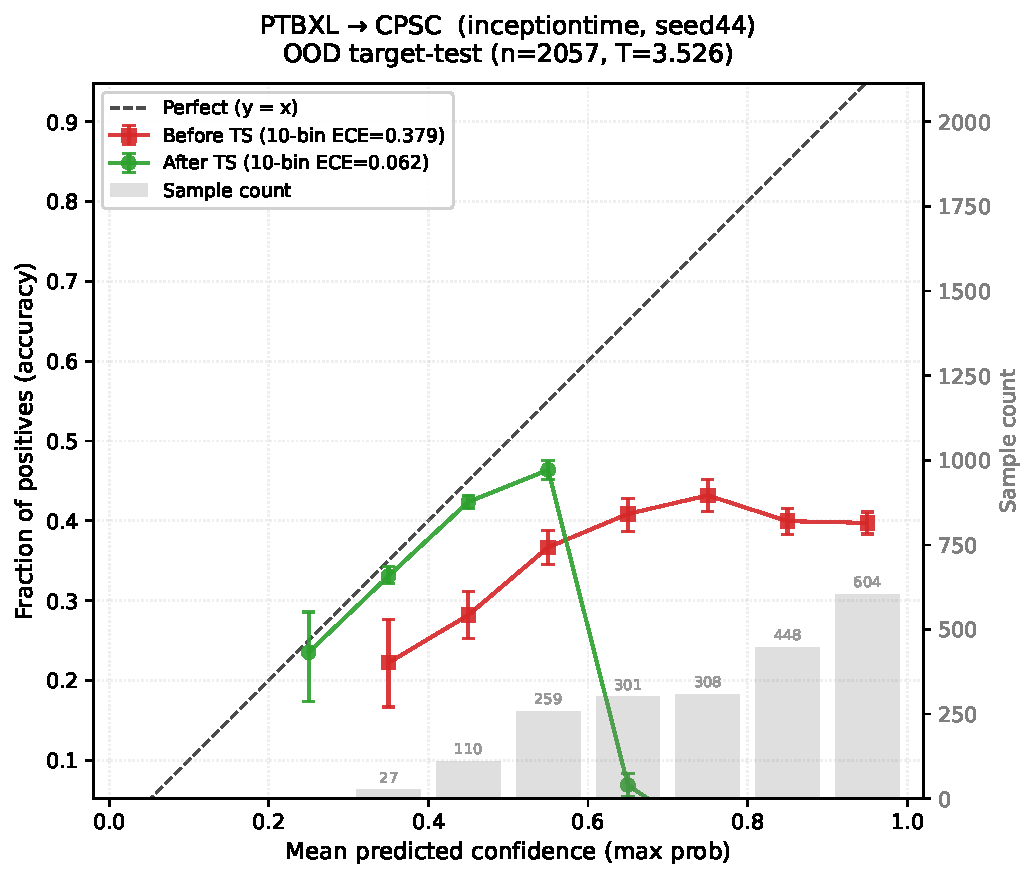
\includegraphics[width=0.32\textwidth]{figures/fig_reliability_supp_ptbxl_cpsc_inceptiontime_seed44.pdf}
\caption{PTB-XL$\to$CPSC reliability diagrams: InceptionTime seeds 42--44.}
\end{figure}

\begin{figure}[h]
\centering
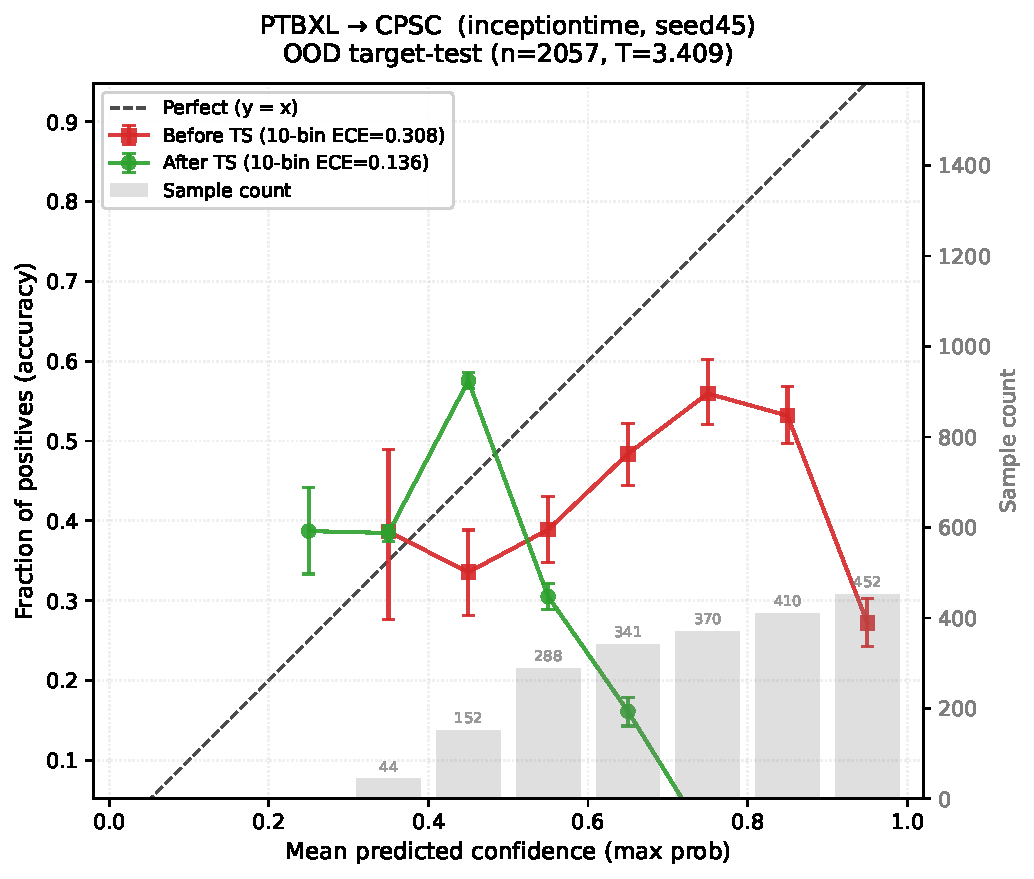
\includegraphics[width=0.45\textwidth]{figures/fig_reliability_supp_ptbxl_cpsc_inceptiontime_seed45.pdf}
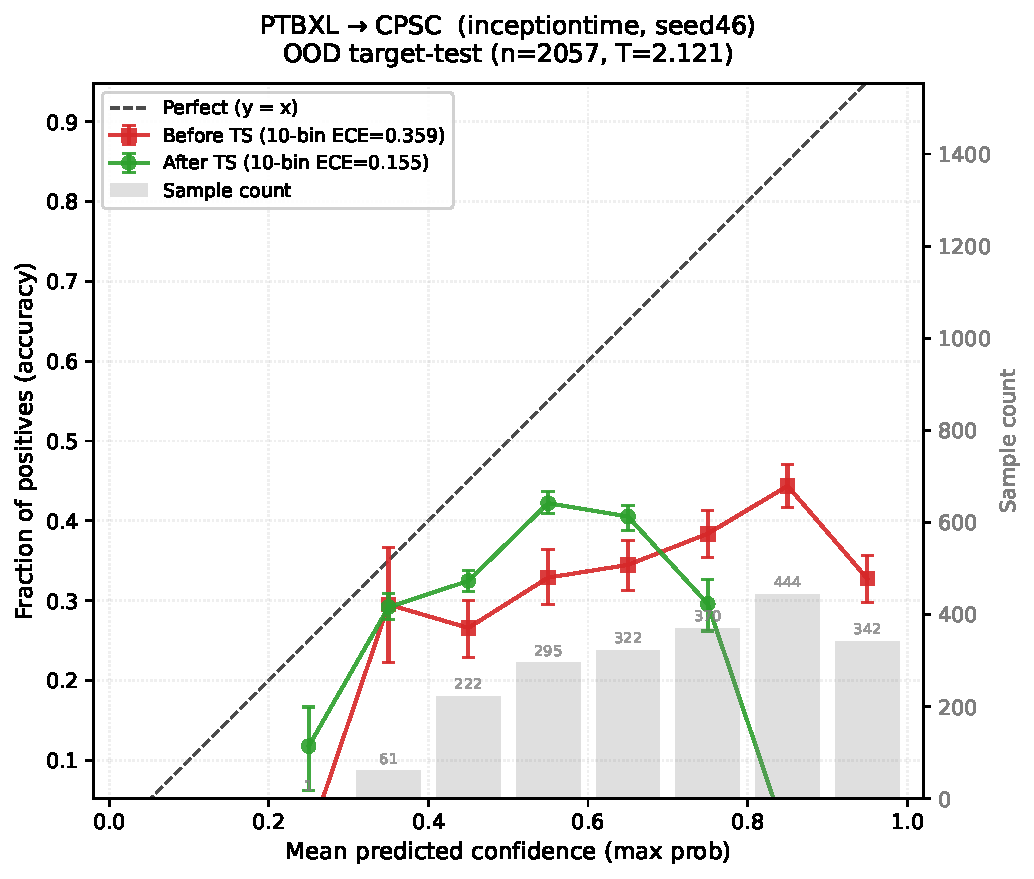
\includegraphics[width=0.45\textwidth]{figures/fig_reliability_supp_ptbxl_cpsc_inceptiontime_seed46.pdf}
\caption{PTB-XL$\to$CPSC reliability diagrams: InceptionTime seeds 45--46.}
\end{figure}

\subsection*{S2.\ Additional supplementary materials}
\label{sec:supp-additional}
\begin{itemize}
    \item \textbf{Per-experiment result files}: full JSON results
    (\texttt{checkpoints/transfer/**/}\allowbreak\texttt{transfer\_result.json})
    and CSV summaries (\texttt{results/*.csv}) for all 60 seed experiments.
    \item \textbf{Pre-registered protocol}: immutable public archive
    with per-file SHA-256 checksums, including the revision A1 full
    text (\url{https://doi.org/10.17605/OSF.IO/53H64}).
    \item \textbf{NCV experiment data}: E3 CSV containing
    \texttt{ncv\_id} and \texttt{ncv\_ood} columns for the net
    clinical value experiment (main text, decision-curve analysis subsection).
    \item \textbf{Shapley decomposition cells}: 27-cell validation
    table for the Shapley attribution analysis at $n=20{,}000$.
    \item \textbf{BCa CI rerun manifest}: full BCa bootstrap
    ($B=10{,}000$) CI results for the entire $6 \times 2 \times 5
    \times 8$ grid, stored in the \texttt{methods.ts.meta} field of
    each \texttt{transfer\_result.json}.
\end{itemize}

% ============================================================================
\begin{thebibliography}{99}
\raggedright
% ============================================================================
\bibitem{ovadia2019calibration} Y.~Ovadia, E.~Fertig, J.~Ren, Z.~Nado,
D.~Sculley, S.~Nowozin, J.~Dillon, B.~Lakshminarayanan, J.~Snoek,
``Can you trust your model's uncertainty? Evaluating predictive
uncertainty under dataset shift,'' \emph{NeurIPS}, 2019.
arXiv:1906.02530.
\bibitem{guo2017calibration} C.~Guo, G.~Pleiss, Y.~Sun, K.~Weinberger,
``On calibration of modern neural networks,'' \emph{ICML}, PMLR
70:1321--1330, 2017. arXiv:1706.04599.
\bibitem{wagner2020ptbxl} P.~Wagner, N.~Strodthoff, R.-D.~Bousseljot,
et al., ``PTB-XL, a large publicly available electrocardiography
dataset,'' \emph{Scientific Data}, 7:154, 2020.
doi:10.1038/s41597-020-0495-6.
\bibitem{zheng2022ecgarrhythmia} J.~Zheng, J.~Guo, H.~Chu,
``A large scale 12-lead electrocardiogram database for arrhythmia
study (Chapman-Shaoxing e-cardiology),'' version 1.0.0,
\emph{PhysioNet}, 2022. doi:10.13026/wgex-er52.
\bibitem{goldberger2000} A.~L. Goldberger et al., ``PhysioBank,
PhysioToolkit, and PhysioNet: components of a new research resource
for complex physiologic signals,'' \emph{Circulation},
101(23):e215--e220, 2000.
\bibitem{nixon2019} J.~Nixon, M.~W. Dusenberry, L.~Zhang, et al.,
``Measuring calibration in deep learning,'' \emph{CVPR Workshops},
pp.~38--41, 2019. arXiv:1904.01685.
\bibitem{kull2019dirichlet} M.~Kull, M.~Perello-Nieto, M.~Kangse,
T.~S.~Filho, P.~Song, P.~Flach, ``Beyond temperature scaling:
obtaining well-calibrated multi-class probabilities with Dirichlet
calibration,'' \emph{NeurIPS}, 2019. arXiv:1910.12656.
\bibitem{alexandari2020} A.~Alexandari, A.~Kundaje, A.~Shrikumar,
``Maximum likelihood with bias-corrected calibration is hard-to-beat
at label shift adaptation,'' \emph{ICML}, PMLR 119:222--232, 2020.
arXiv:1901.06852.
\bibitem{lipton2018bbs} Z.~Lipton, Y.-X.~Wang, A.~Smola,
``Detecting and correcting for label shift with black box
predictors,'' \emph{ICML}, PMLR 80:1944--1953, 2018.
arXiv:1802.03916.
\bibitem{barandas2023} M.~Barandas, L.~Famiglini, A.~Campagner,
D.~Folgado, R.~Sim\~ao, F.~Cabitza, H.~Gamboa, ``Evaluation of
uncertainty quantification methods in multi-label classification: a
case study with automatic diagnosis of electrocardiogram,''
\emph{Information Fusion}, 101:101978, 2024.
doi:10.1016/j.inffus.2023.101978.
\bibitem{zhang2022} J.~F.~Vranken et al., ``Uncertainty estimation for
deep learning-based automated analysis of 12-lead
electrocardiograms,'' \emph{European Heart Journal -- Digital Health},
2(3):423--434, 2021. doi:10.1093/ehjdh/ztab045.
\bibitem{reyna2022} M.~Reyna, N.~Strodthoff, P.~Wagner, et al.,
``Issues in the automated classification of multilead ECGs using
heterogeneous labels and populations,'' \emph{Physiological
Measurement}, 43(8):084001, 2022. doi:10.1088/1361-6579/ac79fd.
\bibitem{efron1987bca} B.~Efron, ``Better bootstrap confidence
intervals,'' \emph{Journal of the American Statistical Association},
82(397):171--185, 1987. doi:10.1080/01621459.1987.10478410.
\bibitem{vancalster2016} B.~Van Calster, D.~J.~Steyerberg,
S.~Collins, R.~D.~Riley, E.~W.~Steyer, ``A calibration hierarchy for
risk models was defined: from utopia to empirical data,''
\emph{Journal of Clinical Epidemiology}, 74:167--176, 2016.
doi:10.1016/j.jclinepi.2015.12.005.
\bibitem{vancalster2019} B.~Van Calster, D.~J.~McLernon,
M.~van~Smeden, L.~Wynants, G.~S.~Collins, ``Calibration: the Achilles
heel of predictive analytics,'' \emph{BMC Medicine}, 17:230, 2019.
doi:10.1186/s12916-019-1466-7.
\bibitem{kumar2019} A.~Kumar, P.~Liang, T.~Ma, ``Verified uncertainty
calibration,'' \emph{NeurIPS}, 2019. arXiv:1909.10155.
\bibitem{strodthoff2021} N.~Strodthoff, P.~Wagner, T.~Schaeffter,
W.~Samek, ``Deep learning for ECG analysis: benchmarks and insights
from PTB-XL,'' \emph{IEEE Journal of Biomedical and Health
Informatics}, 25(5):1519--1528, 2021.
doi:10.1109/JBHI.2020.3022989.
\bibitem{physiolmeas2026} M.~Haekal, S.~N.~Khotimah,
G.~R.~F.~Suwandi, F.~Haryanto, ``RR-interval-based atrial fibrillation
detection and burden estimation: cross-dataset validation and
calibration-aware probability analysis,'' \emph{Physiological
Measurement}, 2026. doi:10.1088/1361-6579/ae99aa.
\bibitem{medrxiv2026} K.~Patel, P.~Beedala, ``Calibration drift under
cross-institutional deployment: an external validation framework for
ICU mortality prediction across MIMIC-IV and eICU,'' \emph{medRxiv}
(preprint), 2026. doi:10.64898/2026.05.03.26352335.
\bibitem{transcal2020} X.~Wang, M.~Long, J.~Wang, M.~I.~Jordan,
``TransCal: transferability estimation for auto-selecting transfer
calibration,'' \emph{NeurIPS}, 2020. arXiv:2007.08259.
\bibitem{pseudocal2020} S.~Garg, Y.~Wu, S.~Balakrishnan, Z.~Lipton,
``A unified view of label shift estimation,'' \emph{NeurIPS}, 2020.
arXiv:2003.07554.
\bibitem{lascal2024} T.~Popordanoska, G.~Radevski, T.~Tuytelaars, et al.,
``LaSCal: label-shift calibration for uncertainty quantification,''
\emph{NeurIPS}, 2024.
\bibitem{morenotorres2012} J.~T.~Moreno-Torres, T.~Raeder,
R.~Alaiz-Rodriguez, N.~Chawla, F.~Herrera, ``A unifying view on
dataset shift in classification,'' \emph{Pattern Recognition},
45(1):521--530, 2012. doi:10.1016/j.patcog.2011.05.019.
\bibitem{protocolv21a1} [Pre-registered protocol, publicly archived] ``ECG
calibration boundary study -- experiment protocol,'' 2026. Immutable
public archive with per-file SHA-256 checksums:
\url{https://doi.org/10.17605/OSF.IO/53H64} (including revision A1 full
text).
\bibitem{nosek2019prereg} B.~Nosek, C.~Ebersole, A.~DeHaven,
D.~Mellor, ``The preregistration revolution,'' \emph{PNAS},
115(11):2600--2606, 2018. doi:10.1073/pnas.1708274114.
\bibitem{lakens2019prereg} D.~Lakens, ``The practical alternative to
the $p$ value is the correctly used $p$ value,''
\emph{Perspectives on Psychological Science}, 16(3):639--648, 2021.
doi:10.1177/1745691620958012.
\bibitem{ecgfounder2024} J.~Li, A.~D.~Aguirre, V.~M.~Junior, et al.,
``An Electrocardiogram Foundation Model Built on over 10 Million
Recordings,'' \emph{NEJM AI},
2(7):AIoa2401033, 2025. doi:10.1056/AIoa2401033.
\bibitem{ecgfm2024} J.~C.~McHugh, B.~Wang, et al., ``ECG-FM: an open
electrocardiogram foundation model,'' \emph{arXiv preprint}
2408.05178, 2024.
\bibitem{heartlang2025} J.~Jin, et al., ``Reading your heart: learning
ECG words and sentences via pre-training ECG language model
(HeartLang),'' \emph{ICLR}, 2025. arXiv:2502.10707.
\bibitem{transferecg2025} C.~V.~Nguyen, C.~D.~Do, ``Transfer learning in ECG
diagnosis: is it effective?'' \emph{PLOS ONE}, 20(5):e0316043, 2025.
doi:10.1371/journal.pone.0316043.
\bibitem{adaptood2026} S.~Vavaroutas, et al., ``ADAPTOOD:
uncertainty-aware fine-tuning for out-of-distribution ECG time series
models,'' \emph{arXiv preprint} 2606.04164, 2026.
\bibitem{beatrhythm2026} W.~Jiang, et al., ``Test-time adaptation for ECG
classification via SQI-gated self-training and beat-rhythm
consistency,'' \emph{arXiv preprint} 2608.23347, 2026 (accepted at
MICCAI 2026).
\bibitem{star2025} N.~Nemati, ``Comparative analysis of data
augmentation for clinical ECG classification with STAR (Sinusoidal
Time--Amplitude Resampling),'' \emph{arXiv preprint} 2510.24740, 2025.
\bibitem{peace2026} X.~Liu, et al., ``PEACE: knowledge-guided
cross-modal fusion for adult-to-pediatric ECG transfer via
label-conditioned contrastive alignment,'' \emph{arXiv preprint}
2605.00647, 2026.
\bibitem{song2024ecgfm} J.~Song, J.-H.~Jang, B.~T.~Lee, D.~Hong,
J.~Kwon, Y.-Y.~Jo, ``Foundation models for electrocardiograms,''
\emph{arXiv preprint} 2407.07110, 2024.
\end{thebibliography}


\end{document}
